
\chapter{Aerial Refueling Scheduling of Multi-Receiver and Multi-Tanker under Spatial-Temporal Constraints}

 Given the constrained load capacities of these aircraft, aerial refueling becomes crucial to extend their operational time and range. Firstly, a fuel consumption calculation model for aerial refueling scheduling is established based on the receiver path. Then, two distinct methods, including an integrated one and a decomposed one, are designed to address the challenges of establishing refueling airspace and allocating tasks for tankers. Both methods aim to optimize total fuel consumption of the receivers and tankers within the aerial refueling scheduling framework. The optimization problem is established as nonlinear optimization models along with restrictions. The integrated method seamlessly combines refueling rendezvous point scheduling and tanker task allocation into unified process. It has a complete solution space and excels in optimizing total fuel consumption. The decomposed method, through the separation of rendezvous point scheduling and task allocation, achieves a reduced computational complexity. However, this comes at the cost of sacrificing optimality by excluding specific feasible solutions. Finally, numerical simulations are carried out to verify the feasibility and effectiveness of the proposed methods. These simulations yield insights crucial for the practical engineering application of both the integrated and decomposed methods in real-world scenarios.

\section{Introduction}
%Forest fires lead to the destruction of the ecological environment and pose significant threats to human life and property safety. \cite{yuan2015survey}Firefighters have primarily relied on traditional methods to extinguish fires so far. For instance, a catastrophic forest fire in Sichuan Province, China suddenly changed direction, resulting in the deaths of 27 firefighters and 4 other individuals. \cite{yu2021fault}The development of modern aviation presents tremendous potential for applications in forest firefighting, offering a substantial reduction in personnel casualties. To carry as many fire-extinguishing retardants as possible for continuous firefighting, fireextinguishing aircraft will take very lim-ited fuel to take off safely, subject to the constraints of the limited load capability and time-saving operation for the firefighting mission. Thus, aerial refueling can extend the operating time, range, and endurance of the aircraft mainly for forest firefighting, providing greater capacity for fire-extinguishing retardants. 

Recently, aerial refueling, particularly Autonomous Aerial Refueling (AAR), has drawn increasing attention from academia and industry, significantly impacting civil and military aviation. \cite{thomas2014advances,ro2011dynamics,yin2022hose,dai2016modeling,tsukerman2018optimal}Thomas et al. conducted a comprehensive review of the present and future aspects of aerial refueling, including modeling, sensors, control strategies, as well as simulation and test. \cite{thomas2014advances}Aerial refueling research refers to many aviation techniques, such as dynamic, modeling, and simulation, \cite{ro2011dynamics,yin2022hose,dai2016modeling,tsukerman2018optimal}path scheduling, \cite{oh2013rendezvous,hansknecht2023feeder}docking control,\cite{quan2014survey,duan2020bionic,valasek2017fault,jinrui2020docking}drogue detection, \cite{rasol2023n,wang2017drogue}mission scheduling, \cite{hansknecht2023feeder,sundar2013algorithms}etc. However, few pieces of research concentrate on scheduling problems, \cite{hao2021autonomous}despite the crucial role they play in aerial refueling. In detail, aerial refueling scheduling is a decision-making problem of coordinating tankers and receivers according to the demand of the receivers subject to limited resources. In general, scheduling technology can significantly enhance aerial refueling efficiency, such as saving time for the key mission, reducing fuel consumption, ensuring refueling safety, increasing resource utilization, etc.

Since the 1880s, with the extensive deployment of aerial refueling capability in U.S. military aircraft, American scholars took the lead in the Aerial Refueling Scheduling Problem (ARSP) research. Bordelon proposed the determinants of the optimal aerial refueling rendezvous point, optimal takeoff fuel load, and minimum fuel carrying capacity. \cite{bordelon1981optimization}This supported the mathematical modeling method to solve the optimization problem for aerial refueling. Many research endeavors have been devoted to improving the ARSP model with larger scales and more practical hypotheses, such as a mathematical model for multi-receiver and single tanker scenario, \cite{liu2019optimal} scheduling solutions for a fleet of airplanes, \cite{gamzu2019polynomial,entz2015application}parallel machine scheduling by heuristic algorithms\cite{kaplan2012exact} and a Deep Reinforcement Learning (DRL) based method for multi-receiver and multi-tanker. \cite{zhu2022aerial}These studies assume that the rendezvous points or the tanker's trajectory are known in advance and focus on refueling task allocation only. Additionally, some researches concentrated only on path planning for the aerial refueling problem, such as an adapted labeling algorithm for multi-tanker, \cite{hansknecht2023feeder}and an approximated fast heuristics algorithm for a single Unmanned Aerial Vehicle (UAV). \cite{sundar2013algorithms}

Many mature algorithms have been developed for task allocation of different vehicles.\cite{kim2018traveling,carter2006new} Some optimiza-tion problems are similar to aerial refueling scheduling, such as refueling path scheduling for the UAVs by the mobile Ground Vehicle (GV), \cite{maini2019cooperative} or the mobile charging vehicles. \cite{1021875904.nh,huang2020planning}In Ref. \cite{maini2019cooperative}, the GV can act as the mobile refueling station for the UAVs. Then, a two-stage method by Mixed-Integer Linear Programming (MILP) was designed for Coverage Path Planning (CPP) missions for coupled UAV-GV. Spatial-temporal networks\cite{1021875904.nh} and Mixed-Integer Nonlinear Programming (MINLP)\cite{huang2020planning} were adopted to solve the scheduling problem of mobile charging vehicles.

The aerial refueling scheduling result requires a balance between safety and efficiency. The drawbacks of the existing research can be summarized as follows. (A) There is a lack of studies that specifically focus on the problem of multiple tankers for multiple receivers, which is crucial in meeting today's extensive aerial refueling requirements. (B) Most studies used the total operating time as the optimization index,\cite{kaplan2012exact} but in forest fire-fighting practice, economics, such as the fuel consumption, is of great importance as well. (C) Almost all of the current studies concentrated on only one aspect of aerial refueling scheduling problem like mathematical modeling,\cite{liu2019optimal}path planning,\cite{hansknecht2023feeder,sundar2013algorithms} rendezvous point scheduling\cite{bordelon1981optimization} or task allocation.\cite{kaplan2012exact,zhu2022aerial} Multi-receiver and multi-tanker studies generally only focused on the task allocation of tankers and assumed that the refueling missions are known in advance. However, receiver's path, rendezvous points, and task allocation are coupled with the total fuel consumption in aerial refueling. Therefore, a mere combination of the existing studies cannot lead to the optimal solution for the multi-receiver and multi-tanker aerial refueling scheduling problem, specifically aiming to minimize fuel consumption.

In this paper, multiple support tankers from the multiple takeoff and landing airports. Many challenges are involved, such as minimum and maximum fuel load constraints, threat areas, etc. The aerial refueling scheduling problem is cast into a task allocating model with spatial-temporal constraints. Because the functions of fuel consumption and spatial-temporal constraints in the problem are nonlinear, the optimization for the rendezvous points and initial fuel load is a nonlinear programming problem which is difficult to solve. Thus, in the simulations, the Genetic Algorithm (GA) is employed to obtain the approximate optimal solution to such a nonlinear NP-hard problem. The main contributions of this work can be outlined as follows:

(1) For large-scale AAR requirements, the aerial refueling scheduling problem is studied in the scenario of multiple receivers and tankers, multiple airports, and long-range operations of receivers.

(2) Mathematical modeling, rendezvous points scheduling, path planning and task allocation are integrated, and the total fuel consumption is employed as the optimization index.

(3) Two aerial refueling scheduling methods with multiple receivers and tankers are proposed. In the integrated method, the rendezvous points and task allocation are scheduled simultaneously. A decomposed scheduling method is further designed for less calculation time by decoupling the whole optimization process into two independent processes: rendezvous point scheduling and task allocation. Simulation tests are carried out to compare the efficiency of the developed methods.

The remainder of this paper is organized as follows. Section \ref{sec_2} generalizes the aerial refueling mission for multi-receiver and multi-tanker and formulates scheduling models and fuel consumption models for the aircraft. Section \ref{sec_3} gives the scheduling flow and the path planning algorithm based on A* algorithm. In Section \ref{sec_4}, the integrated and decomposed scheduling methods are proposed to obtain the optimal refueling solution. In Section \ref{sec_5}, the proposed methods are testified by the simulation of aerial refueling scheduling problems with several receivers and tankers.

The notations used in this paper are summarized in Table \ref{Tab_15.1}.

\begin{table}
	\caption{Definition of main notations}
	
	\begin{centering}
		\begin{tabular}{|c|c|}
			\hline 
			Notation & Meaning\tabularnewline
			\hline 
			${N_\text{r}},{N_\text{t}}$ & Receiver number, tanker number\tabularnewline
			
			$\left\{\mathbf{p}_{\text{r},i_\text{r},i}\right\}_{i=0}^{N_{i_\text{r}}},\left\{\mathbf{p}_{\text{r}^{\prime},i_\text{r},i}\right\}_{i=0}^{N_{i_\text{r}}}$ & Departure path, return path of the $i_{\text{r}}^{\text{th}}$ receiver\tabularnewline
			
			$\left\{\mathbf{p}_{\text{t},i_{\text{t}},0},\mathbf{p}_{\text{t},i_{\text{t}},1},\cdots,\mathbf{p}_{\text{t},i_{\text{t}},k_{i_\text{t}}},\mathbf{p}_{\text{t},i_{\text{t}},0}\right\}$& Path of the $i_{\text{t}}^{\text{th}}$ tanker\tabularnewline
			
			$F_{_{\text{r},i_{\text{r}}}},F_{_{\text{t},i_{\text{t}}}}$ & Total fuel consumption mass of the $i_{\text{r}}^{\text{th}}$ receiver, the $i_{\text{t}}^{\text{th}}$ tanker\tabularnewline
			
			$F_{\text{r,tk}},F_{\text{r,ld}},F_{\text{r,rfl}},F_{\text{r,}i_\text{r},\text{tsk}}$ & Fuel consumption mass during the takeoff, landing, refueling, task process of the receiver\tabularnewline
			
			$F_{_{\text{r},d_{i_\text{r}},i}}$ & Fuel consumption mass during the $i_{}^{\text{th}}$ flight segment of the $i_{\text{r}}^{\text{th}}$ receiver\tabularnewline
			
			$F_{\text{r},i_{\text{r}},\text{rfl},1},F_{\text{t},i_{\text{t}},\text{rfl},2}$ & Received fuel mass during the first refueling, second refueling of the $i_{\text{r}}^{\text{th}}$ receiver\tabularnewline
			
			$F_{\text{t,tk}},F_{\text{t,ld}},F_{\text{t,rfl}}$ & Fuel consumption mass during the takeoff, landing, refueling process of a tanker\tabularnewline
			
			$F_{\text{t},d_{i_\text{t}},i},F_{\text{t},i_\text{t},{i},\text{wt}}$ & Fuel consumption mass during the $i_{}^{\text{th}}$ flight segment, hovering and waiting process of the $i_{\text{t}}^{\text{th}}$ tanker\tabularnewline
			
			$F_{\text{t},i_{\text{t}},i,\text{rfl}}$ & Served fuel mass during the $i_{}^{\text{th}}$ refueling of the $i_{\text{t}}^{\text{th}}$ tanker\tabularnewline
			
			$F_{\text{r,min}},F_{\text{r,max}},F_{\text{t,min}},F_{\text{t,max}}$ & Minimum and maximum safe fuel load mass of receiver and tanker\tabularnewline
			
			
			$\mathbf{P}_{\text{ob}},\mathbf{P}_{\text{s}}$ & Obstacle airspace set, safe airspace set\tabularnewline
			$\mathbf{k}_{\text{1}},\mathbf{k}_{\text{2}}$ & Waypoint serial numbers of the first and second aerial refueling rendezvous points\tabularnewline
			
			$\mathbf{n}_{\text{1}},\mathbf{n}_{\text{2}}$ & Tankers'serial numbers allocated to the first and second refueling missions of the receivers\tabularnewline
			
			$\mathbf{X},\mathbf{Y},K$ & Refueling mission grouping matrix, refueling mission allocation matrix, number of refueling mission group\tabularnewline
			
			\hline 
		\end{tabular}
		\par\end{centering}
	\centering{}\label{Tab_15.1}
\end{table}



\section{Problem formulation}\label{sec_2}

\subsection{Aerial refueling mission}

\begin{figure}
	\begin{centering}
		\includegraphics[width=0.8\textwidth]{Figures/Figs_Ch16/Fig_15\lyxdot 1}
		\par\end{centering}
	\caption{Schematic diagram of aerial refueling scheduling problem by multiple receivers and tankers.}
	
	\centering{}\label{Fig_15.1}
\end{figure}

Fig. \ref{Fig_15.1} is a schematic diagram of the aerial refueling scheduling problem by multiple receivers and tankers. In an aerial refueling problem, there are two different kinds of controlled objects: tankers and receivers. The optimization objective is to minimize the overall fuel consumption of receivers and tankers under the prerequisite that the receivers fly to and from the task area safely and accurately. As shown in Fig.\ref{Fig_15.1}, the whole airspace is divided into two by a black solid line. The left area is the safety zone, while the right area represents the task zone, which is deemed unsafe for tankers due to complex updraft. Aerial refueling can only be performed in the safety zone to guarantee safety. The left slash and right slash ellipses are the refueling and threat areas, respectively. The round, triangle, square nodes and pentagon, rhombus, hexagon, trapezoid with different numbers represent the waypoints of different receivers and tankers. Correspondingly, the different kinds of lines passing through them are the flight paths of different tankers and receivers. The solid circles are airports located in the safety zone. The whole flight process of the receiver'  operation is presented as follows: several receivers take off from the airports and perform the first aerial refueling operations when reaching the corresponding aerial refueling points. Then, they fly to the task areas and perform task. After that, they return to refueling points by following the planned path for the second aerial refueling operation. Finally, they return to the landing airports. Accordingly, the complete flight process of the tankers is given as follows: departing from the airport, flying through all aerial refueling mission points following the order of the sorted aerial refueling missions, completing each refueling, and finally, returning to the landing airport.






















\subsection{Basic assumptions}

According to various complex factors of aerial refueling mission requirements, the aerial refueling mission model established in this paper is based on the following assumptions:\\
\textbf{Assumption 1.} Only fuel can be transferred by aerial refueling.\\
\textbf{Assumption 2.}  Each receiver will be refueled twice in the whole round trip: the first one is on its departure path to guarantee enough fuel from the takeoff airport to reach the task area, and the second one is on its returning path to ensure enough fuel from the task area to the landing airport. One-to-one rendezvous approach is employed for the refueling between the tanker and the receiver.\\\textbf{Assumption 3.}  Since the refueling areas are set in the safe zone, all the flight paths of tankers will not be ex-posed to threats. Therefore, the tankers will fly according to the great circle paths between airports and each aerial refueling mission point.\\
\textbf{Assumption 4.}  The fuel consumption of each aircraft in the takeoff and landing phases is taken into account according to the average fuel consumption.\\
\textbf{Assumption 5.}  The aircraft flies at cruise speed during the whole operating process, and the altitude and speed of the aircraft are unchanged. The earth is an ideal sphere with a radius $R=6371 \text{km}$ . The tanker and the receiver fly at a fixed cruising speed between the two waypoints with a fixed altitude $H=5 \text{km}$ . Aircraft fly between two path points in the air according to the great circle paths. \\
\textbf{Assumption 6.}  Tankers and receivers fly in the stratosphere, ignoring the influence of weather, wind direction, and wind speed.

The coordinate position is expressed by latitude and longitude. The equation for calculating the distance of the great circular arc between the starting point and the ending point is given as follows:
\begin{equation}
\left.d\left(\mathbf{p}_{1},\mathbf{p}_{2}\right.\right)=\left(R+H\right)\cos^{-1}\left(\sin\beta_{1}\sin\beta_{2}+\cos\beta_{1}\cos\beta_{2}\right)\cos\left(\alpha_{2}-\alpha_{1}\right)
\label{eq:15.1}
\end{equation}
where $\mathbf{p}_{1},\mathbf{\textbf{p}}_{2}\in\mathbb{R}^{2}$ are the coordinates of starting and ending points on the path, $\alpha_{1},\beta_{1}\in\mathbb{R}$ are the latitude and longitude coordinates of the starting point, and $\alpha_{2},\beta_{2}\in\mathbb{R}$ are the latitude and longitude coordinates of the ending point.

The coordinates of the starting point and the ending point are given as follows:
\begin{equation}
\begin{cases}\mathbf{p}_{1}=\left[\alpha_1\ \beta_1\right]^{\text{T}}\\\mathbf{p}_2=\left[\alpha_2\ \beta_2\right]^{\text{T}}\end{cases}
\label{eq:15.2}
\end{equation}	

\subsection{Scheduling models}
\subsubsection{Fuel consumption model}\label{sec_2.3.1}

In this paper, the fuel consumption models of receivers and tankers adopt the nonlinear fuel consumption calculation equation to increase the model's authenticity. Because the fuel consumption of various aircraft is very complex and the parameter selection should be adjusted according to the specific situation, to simplify the calculation, a simplified model of the aerial refueling fuel consumption is employed in this paper.

The fuel consumption mass per unit distance of an aircraft at a specific flight altitude is given as follows:
\begin{equation}
f(G)=\frac{q}{G}
\label{eq:15.3}
\end{equation}	  
where $G\in\mathbb{R}$ represents the total weight of the aircraft, and $q\in\mathbb{R}$ represents the fuel coefficient of aircraft. The total weight of the aircraft includes the empty weight and carried load weight as follows:    
\begin{equation}
G=\left(m_\text{0}+m_\text{c}\right)g
\label{eq:15.4}
\end{equation}	  
where $m_\text{0}\in\mathbb{R}$ is the empty mass of the aircraft, $m_\text{c}\in\mathbb{R}$ is the carried load mass which is variable during flight, and $g\in\mathbb{R}$ is the acceleration of gravity. The fuel consumption mass function concerning the remaining fuel mass is given as follows:\cite{marchman2004aerodynamics}

\begin{equation}
F^{\prime}\left(m_{\text{rl}},d\right)=\left(m_\text{0}+m_{\text{rl}}\right)\left(\text{e}^{\frac dq}-1\right)
\label{eq:15.5}
\end{equation}	 
where $m_\text{rl}\in\mathbb{R}$ is the remaining carried load.

Assuming that the carried load of the aircraft is only fuel, $m_\text{f,max}\in\mathbb{R}$ is the maximum carried fuel mass when it takes off, and $d_\text{max}\in\mathbb{R}$ is the maximum flight distance. Substituting $F^{\prime}(m_{\text{rl}},d)=m_{\text{f,max}},m_{\text{rl}}=0\text{~kg}$ and $d=d_\text{max}$ into Eq.\ref{eq:15.5}, we can obtain the fuel coefficient calculating formula as follows:

\begin{equation}
q=\frac{d_\text{max}}{\ln(m_\text{f,max}+m_0)-\ln m_0}
\label{eq:15.6}
\end{equation}	

The carried loads of a tanker in the aerial refueling mission are all fuel, while the carried loads of a receiver are composed of two parts: fuel and ammunition. The fuel consumption mass equations of receivers and tankers concerning the remaining fuel mass are given as follows:

\begin{equation}
F_\text{r}^{\prime}\big(m_1,m_\text{rf},d\big)=\text{e}^{\ln\left(m_\text{r0}+m_1+m_\text{rf}\right)+d/q_\text{r}}-\big(m_\text{r0}+m_1+m_\text{rf}\big)
\label{eq:15.7}
\end{equation}	 

\begin{equation}
F_{\text{t}}^{\prime}(m_{\text{rf}},d)=\text{e}^{\ln(m_{\text{t}0}+m_{\text{tf}})+d/q_{\text{t}}}-\left(m_{\text{t}0}+m_{\text{rf}}\right)
\label{eq:15.8}
\end{equation}	 
where $m_\text{1}\in\mathbb{R}$ is the carried load mass of ammunition, $m_\text{r0},m_\text{t0}\in\mathbb{R}$ are the empty mass of the receiver and the tanker, respectively, and $q_\text{r},q_\text{t}\in\mathbb{R}$ are the fuel coefficient of the receiver and the tanker, respectively.







\subsubsection{Dynamic model}

Fig. \ref{Fig_15.2} depicts the relative geometry between a receiver and a tanker. In Fig.\ref{Fig_15.2}, $\psi_{\text{r}},\psi_{\text{t}}\in\mathbb{R}$ are the heading angles  of the receiver and the tanker, respectively, $V_{\text{r}},V_{\text{t}}\in\mathbb{R}$ are the speed of the receiver and the tanker, respectively, $\lambda\in\mathbb{R}$ denotes the Line-of-Sight (LOS) angle of the aircraft, and $d_{\text{rt}}\in\mathbb{R}$ denotes the distance between a receiver and a tanker. 

\begin{figure}
	\begin{centering}
		\includegraphics[width=0.8\textwidth]{Figures/Figs_Ch16/Fig_15\lyxdot 2}
		\par\end{centering}
	\caption{Relative geometry between a receiver and a tanker.\cite{yoon2018three}}
	\centering{}\label{Fig_15.2}
\end{figure}



The dynamics of the receiver and the tanker are represented as follows:\cite{yoon2018three}

\begin{equation}
\begin{aligned}&\begin{cases}\dot{d}_\text{r,t}=-V_\text{r}\cos\left(\psi_\text{r}-\lambda\right)+V_\text{t}\cos\left(\psi_\text{t}-\lambda\right)\\\dot{\lambda}=-\left(\frac{V_\text{r}}{d_\text{r,t}}\right)\text{sin}\left(\psi_\text{r}-\lambda\right)+\left(\frac{V_\text{t}}{d_\text{r,t}}\right)\text{sin}\left(\psi_\text{t}-\lambda\right)&\end{cases}\end{aligned}
\label{eq:15.9}
\end{equation}	 


\subsubsection{Obstacle model}
Receivers take off from the takeoff airports according to the sched-ule, arriving at the mission point safely and timely with aerial refueling support of tankers, and the same for the returning path. Receivers need to avoid threat areas distributed near the task areas during the flight paths. Therefore, refueling rendezvous points are constrained spatially by the threat areas. 

The point set of obstacle airspace is given as follows:

\begin{equation}
\mathbf{P}_{\text{ob}}=\left\{\left.\mathbf{p}\in\mathbb{R}^2\right|d\left(\mathbf{p},\mathbf{p}_{\text{c}i}\right)<r_i,i=1,2,\cdots,N_{\text{ob}}\right\}
\label{eq:15.10}
\end{equation}	 
where $\mathbf{p}_{\text{c}i}\in\mathbb{R}^2$ is the center coordinates of the $i^{\text{th}}$ round obstacle area,  $r_{i}\in\mathbb{R}$ is the radius of the round obstacle area, and $N_{\text{ob}}\in\mathbb{N}$ represents the number of obstacles.

\subsubsection{Path model}
The flight path in this paper is given in the form of the following sequential coordinate points set:
\begin{equation}
\left\{\mathbf{p}_i\right\}_{i=0}^{N_{\mathbf{p}}}=\left\{\mathbf{p}_{0},\mathbf{\textbf{p}}_{1},\cdots,\mathbf{p}_{N_{\text{p}}-1},\mathbf{p}_{N_{\text{p}}}\right\}
\label{eq:15.11}
\end{equation}	 
where $\mathbf{p}_{i},i=0,1,\cdots,N_{\text{p}}$ represent the $i^{\text{th}}$ point coordinates in the flight path, $\mathbf{p}_{0},\mathbf{p}_{N_\text{p}}$ represent the coordinates of the starting point and the ending point, respectively, and $N_\text{p}\in\mathbb{N}$ represents the number of waypoints in the path.

The flight path of a receiver from its takeoff airport to its landing airport is separated into two parts: the flight path of the receiver from its takeoff airport to the target point, and the flight path of receiver from the target point to the landing airport. According to the notations above, where  $\left\{\mathbf{p}_{\text{r},i_\text{r},i}\right\}_{i=0}^{N_{i_\text{r}}},{i}_{\text{r}}=1,2,\cdots,N_{\text{r}}$  represents the departure path of the $i_{\text{r}}^{\text{th}}$ receiver,  $\left\{\mathbf{p}_{\text{r}^{'},i_\text{r},i}\right\}_{i=0}^{N_{i_\text{r}}^{'}},{i}_{\text{r}}=1,2,\cdots,N_{\text{r}}$  represents the returning path of the $i_{\text{r}}^{\text{th}}$  receiver, $N_{i_\text{r}}$  and $N_{i_\text{r}}^{'}$  represent the total waypoint number of the departure and returning flight path of the  $i_{\text{r}}^{\text{th}}$  receiver, respectively, and  $N_\text{r}\in\mathbb{N}$ is the number of receivers. The flight path of a tanker depends on the coordinates of its takeoff airport. The path $\left\{\mathbf{p}_{\text{t},i_{\text{t}},0},\mathbf{p}_{\text{t},i_{\text{t}},1},\cdots,\mathbf{p}_{\text{t},i_{\text{t}},k_{i_{\text{t}}}},\mathbf{p}_{\text{t},i_{\text{t}},0}\right\},i_{\text{t}}=1,2,\cdots,N_{\text{t}}$  is selected as the flight path of the $i_{\text{t}}^{\text{th}}$  tanker, where $N_\text{t}\in\mathbb{N}$  is the number of tankers, $k_{i_\text{t}}\in\mathbb{N}$  is the number of refueling missions allocated to the $i_{\text{t}}^{\text{th}}$  tanker, and $\mathbf{p}_{\text{t},i_{\text{t}},0}\in\mathbb{R}^{2}$  is the location coordinates of the takeoff and landing airport of the $i_{\text{t}}^{\text{th}}$ tanker.


\subsection{Fuel consumption calculation}
The goal of refueling scheduling is to minimize the total fuel consumption of receivers and tankers under the premise that all aircraft are safe. The calculation methods of the fuel consumption of each receiver and tanker are given in this section. Since the missions and the flight paths of receivers and tankers in the problem are different, the fuel consumption mass of the two objects needs to be modeled separately for calculation.


\subsubsection{Receiver fuel consumption calculation}
Fig. \ref{Fig_15.3} depicts the flight path of a single receiver and two tankers in the aerial refueling scheduling problem. In Fig. \ref{Fig_15.3}, $i_\text{r}\in\left\{1,2,\cdots,N_\text{r}\right\}$ represents the serial number of the receiver, and  $N_\text{r}$ is the total number of receivers; $\mathbf{p}_{\text{r},i_\text{r},\text{tk}},\mathbf{p}_{\text{r},i_\text{r},\text{ld}}\in\mathbb{R}^2$  represent the coordinates of takeoff and landing airport of the $i_{\text{r}}^{\text{th}}$  receiver, respectively; $\mathbf{p}_{\text{r},i_\text{r},\text{tsk}}\in\mathbb{R}^2$  represents the coordinate of the target point of the $i_{\text{r}}^{\text{th}}$ receiver; $\mathbf{p}_{\text{t},\text{tk/ld}}\in\mathbb{R}^2$  represents the takeoff and landing airport of tankers; $\mathbf{p}_{\text{r},i_{\text{r}},k_{i_{\text{r}}},1},\mathbf{p}_{\text{r},i_{\text{r}},k_{i_{\text{r}}},2}\in\mathbb{R}^{2}$  represent the coordinates of the first and second aerial refueling rendezvous points of the $i_{\text{r}}^{\text{th}}$  receiver, respectively, where the number  $k_{{i_\text{r}},1}\in\left\{1,2,\cdots,N_{i_\text{r}}\right\}$ is the waypoint serial number of the first aerial refueling airspace on the departure path of the $i_{\text{r}}^{\text{th}}$  receiver, and  $k_{{i_\text{r}},2}\in\left\{1,2,\cdots,N_{i_\text{r}}^{'}\right\}$ is the waypoint serial number of the second aerial refueling airspace on the returning path of the $i_{\text{r}}^{\text{th}}$  receiver. 

\begin{figure}
	\begin{centering}
		\includegraphics[width=0.8\textwidth]{Figures/Figs_Ch16/Fig_15\lyxdot 3}
		\par\end{centering}
	\caption{Aerial refueling point scheduling with a single receiver.}
	\centering{}\label{Fig_15.3}
\end{figure}

In Fig. \ref{Fig_15.3}, $d_{i_{\text{t}},1},d_{j_{\text{t}},1}\in\mathbb{R}$  represent the flight distances of tankers from the takeoff and landing airport $\mathbf{p}_{\text{t},\text{tk/ld}}$  to the first and second refueling points of the   receiver, respectively, and $d_{i_{\text{t}},2},d_{j_{\text{t}},2}\in\mathbb{R}$   represent the flight distances of tankers from the first and second refueling points of the $i_{\text{r}}^{\text{th}}$ receiver to the airport  $\mathbf{p}_{\text{t},\text{tk/ld}}$ , respectively. The overall flight history of the $i_{\text{r}}^{\text{th}}$   receiver includes five nodes and four flight paths. The lengths of the four paths of the $i_{\text{r}}^{\text{th}}$   receiver are denoted by $d_{i_{\text{r}},1},d_{i_{\text{r}},2},d_{i_{\text{r}},3},d_{i_{\text{r}},4}\in\mathbb{R}$  , respectively. The length $d_{i_{\text{r}},1}$  is the path length of the receiver from the takeoff airport to the first aerial refueling point, $d_{i_{\text{r}},2}$  is the path length of the receiver from the first refueling rendezvous point to the target point,  $d_{i_{\text{r}},3}$ is the path length of the receiver returning from the target point to the second aerial refueling rendezvous point, and $d_{i_{\text{r}},4}$  is the path length of the receiver from the second aerial refueling rendezvous point to the landing airport.
The total fuel consumption of the  $i_{\text{r}}^{\text{th}}$ receiver is the sum of takeoff and landing fuel consumption, fuel consumption of four cruise sections,and fuel consumption of the first and second aerial refueling as follows: 

\begin{equation}
F_{\text{r},i_{\text{r}}}=F_{\text{r},\text{t}\text{k}}+F_{\text{r},d_{i_{\text{r}},\text{l}}}+F_{\text{r},d_{i_{\text{r}},\text{2}}}+F_{\text{r},i_{\text{r}},\text{t}\text{s}\text{k}}+F_{\text{r},d_{i_{\text{r}},\text{3}}}+F_{\text{r},d_{i_{\text{r}},\text{4}}}+2F_{\text{r},\text{r}\text{f}\text{l}}+F_{\text{r},\text{l}\text{d}}
\label{eq:15.12}
\end{equation}	 
Here,\\
(1) $F_{\text{r},\text{t}\text{k}},F_{\text{r},\text{l}\text{d}}\in\mathbb{R}$	are the average fuel consumption mass of a receiver during takeoff and landing, respectively.\\
(2) $F_{\text{r},d_{i_{\text{r}},\text{l}}},F_{\text{r},d_{i_{\text{r}},\text{2}}},F_{\text{r},d_{i_{\text{r}},\text{3}}},F_{\text{r},d_{i_{\text{r}},\text{4}}}\in\mathbb{R}$	  correspond to the fuel consumption mass of four flight segments   $d_{i_{\text{r}},1},d_{i_{\text{r}},2},d_{i_{\text{r}},3},d_{i_{\text{r}},4}$   of the $i_{\text{r}}^{\text{th}}$  receiver, respectively.\\
(3) $F_{\text{r},\text{r}\text{f}\text{l}}\in\mathbb{R}$	  is the expected fuel consumption mass of the $i_{\text{r}}^{\text{th}}$  receiver.\\
(4) $F_{\text{r},\text{r}\text{f}\text{l}}\in\mathbb{R}$	 is the fuel consumption mass of the receiver during one aerial refueling.

According to the waypoint serial numbers of refueling rendezvous airspaces corresponding to the $i_{\text{r}}^{\text{th}}$  receiver's flight paths $k_{i_{\text{r}},1}$  and $k_{i_{\text{r}},2}$ , the path length of each flight segment is calculated by summing the distances between the consecutive path points on the segment as follows:

\begin{equation}
\left.\left\{\begin{aligned}d_{i_\text{r},1}&=\sum_{i=1}^{k_{i_\text{r},1}-1}d\left(\mathbf{p}_{\text{r},i_{\text{r}},i},\mathbf{p}_{\text{r},i_{\text{r}},i+1}\right)\\d_{i_\text{r},2}&=\sum_{i=k_{i_\text{r},1}}^{N_{i_\text{r}}-1}d\left(\mathbf{p}_{\text{r},i_{\text{r}},i},\mathbf{p}_{\text{r},i_{\text{r}},i+1}\right)\\d_{i_\text{r},3}&=\sum_{i=1}^{k_{i_\text{r},2}-1}d\left(\mathbf{p}_{\text{r}^{\prime},i_{\text{r}},i},\mathbf{p}_{\text{r}^{\prime},i_{\text{r}},i+1}\right)\\d_{i_\text{r},4}&=\sum_{i=k_{i_\text{r},2}}^{N_{i_\text{r}}^{\prime}-1}d\left(\mathbf{p}_{\text{r}^{\prime},i_{\text{r}},i},\mathbf{p}_{\text{r}^{\prime},i_{\text{r}},i+1}\right)\end{aligned}\right.\right.
\label{eq:15.13}
\end{equation}	 
where $\mathbf{p}_{\text{r},i_{\text{r}},i},\mathbf{p}_{\text{r}^{\prime},i_{\text{r}},i}\in\mathbb{R}^{2}$  represent the coordinates of the  $i_{}^{\text{th}}$  waypoint coordinates on the departure and returning paths of the $i_{\text{r}}^{\text{th}}$  receiver, respectively. Fig. \ref{Fig_15.4} is the carried fuel amount trend changes diagram of the   $i_{\text{r}}^{\text{th}}$ receiver in the whole flight. As shown in Fig. \ref{Fig_15.4}, the fuel load mass of a receiver is between the minimum and maximum safe fuel load mass $F_{\text{r,min}},F_{\text{r,max}}\in\mathbb{R}$  of the receiver. The aircraft fuel consumption mass rate is positively correlated with the aircraft's total weight. The flight distance of each receiver's flight segment is fixed, and its load mass remains the same on each flight segment. As a result, in each flight segment, the smaller the initial or remaining fuel load mass of the receiver is, the smaller its fuel consumption mass is. To ensure that the receiver is safe, the amount of fuel carried by the receiver should not be less than $F_{\text{r,min}}$  during the flight. Thus, for a purely fuel-consuming phase, the receiver consumes the least fuel when the remaining fuel is equal to $F_{\text{r,min}}$  at the end of the phase.

\begin{figure}
	\begin{centering}
		\includegraphics[width=0.8\textwidth]{Figures/Figs_Ch16/Fig_15\lyxdot 4}
		\par\end{centering}
	\caption{Carried fuel amount trend changes of the $i_{\text{r}}^{\text{th}}$ receiver in whole flight phase.}
	\centering{}\label{Fig_15.4}
\end{figure}

When the amount of the carried fuel mass for the receiver is equal to $F_{\text{r,min}}$  when it lands and before refueling, according to Eq. \ref{eq:15.7}, the minimum aerial refueling mass required at two aerial refueling points and fuel consumption for each path section are derived as follows:

\begin{equation}
\begin{cases}F_{\text{r},d_{i_\text{r},4}}=F_{\text{r}}'\Big(0,F_{\text{r},\text{min}}+F_{\text{r},\text{l}\text{d}},d_{i_\text{r},4}\Big)\\F_{\text{r},i_{\text{r}},\text{r}\text{f}\text{l},2}=F_{\text{r},\text{l}\text{d}}+F_{\text{r},d_{i_\text{r},4}}+F_{\text{r},\text{r}\text{f}\text{l}}\\F_{\text{r},d_{i_\text{r},3}}=F_{\text{r}}'\Big(0,F_{\text{r},\text{min}},d_{i_{\text{r}},3}\Big)\\F_{\text{r},d_{i_\text{r},2}}=F_{\text{r}}^{\prime}\Big(m_{\text{r,}i_{\text{r}},1},F_{\text{r,min}}+F_{\text{r},d_{i_\text{r},3}}+F_{\text{r,tsk}},d_{i_{\text{r}},2}\Big)\\F_{\text{r},i_\text{r},\text{r}\text{f}\text{l},1}=F_{\text{r},d_{i_\text{r},2}}+F_{\text{r},\text{tsk}}+F_{\text{r},d_{i_\text{r},3}}+F_{\text{r},\text{rfl}}\\F_{\text{r},d_{i_\text{r},1}}=F_{\text{r}}^{\prime}\Big(m_{\text{r},i_{\text{r}},l},F_{\text{r},\text{min}},d_{i_{\text{r}},1}\Big)\end{cases}
\label{eq:15.14}
\end{equation}
where $F_{\text{r},i_\text{r},\text{r}\text{f}\text{l},1},F_{\text{r},i_\text{r},\text{r}\text{f}\text{l},2}\in\mathbb{R}$  represent the refueling mass of the $i_{\text{r}}^{\text{th}}$  receiver for two aerial refueling operations, and $ m_{\text{r,}i_{\text{r}},1}\in\mathbb{R} $ represents the load mass of extinguishment retardant carried by the $i_{\text{r}}^{\text{th}}$  receiver.

When the fuel load mass of a receiver is equal to  $F_\text{r,min}$ before the first aerial refueling operation, the takeoff fuel load mass of the $i_{\text{r}}^{\text{th}}$ receiver is derived as follows:

\begin{equation}
F_{\text{r},i_{\text{r}},0}=F_{\text{r},\text{min}}+F_{\text{r},d_{i_{\text{r}},1}}+F_{\text{r},\text{tk}}
\label{eq:15.15}
\end{equation}

In each node of the whole flight for the receiver, the task starting time  $t_{\text{r},i_{\text{r}},\text{tsk}}$ is the only node with a known time, so the time of other nodes can be derived by $t_{\text{r},i_{\text{r}},\text{tsk}}$ . The time spent on the path between the nodes is calculated by the path length and cruise speed of the receiver. The takeoff time of the $i_{\text{r}}^{\text{th}}$  receiver is given as follows:

\begin{equation}
t_{\text{r},i_{\text{r}},0}=t_{\text{r},i_{\text{r}},\text{tsk}}-\frac{d_{i_{\text{r}},1}+d_{i_{\text{r}},2}}{V_{\text{r}}}-T_{\text{rfl}}
\label{eq:15.16}
\end{equation}
where  $T_{\text{rfl}}\in\mathbb{R}$ is the time spent on aerial refueling for one flight.

The first aerial refueling rendezvous time of the $i_{\text{r}}^{\text{th}}$  receiver is given as follows:

\begin{equation}
t_{\text{r},i_{\text{r}},\text{rfl},1}=t_{\text{r},i_{\text{r}},\text{tsk}}-\frac{d_{i_{\text{r}},2}}{V_{_{\text{r}}}}-T_{_{\text{rfl}}}
\label{eq:15.17}
\end{equation}

The second aerial refueling rendezvous time of the receiver is given as follows:

\begin{equation}
t_{\text{r},i_\text{r},\text{rfl},2}=t_{\text{r},i_\text{r},\text{tsk}}+T_{\text{r},i_\text{r},\text{tsk}}+\frac{d_{i_\text{r},3}}{V_\text{r}}
\label{eq:15.18}
\end{equation}
where $T_{\text{r},i_\text{r},\text{tsk}}\in\mathbb{R}$  is the time spent on the  $i_{\text{r}}^{\text{th}}$  receiver to complete its task.

If the task zone is close to the airport, the aircraft can carry enough fuel before takeoff to complete the task, and it is unnecessary to be refueled again. For a receiver with a known route, the method of determining the number of in-flight refueling required is presented below.

\textbf{Remark 1.} If the receiver is not refueled during the entire flight, the fuel consumption from takeoff airport to landing airport should be less than its maximum amount of the carried fuel as follows:

\begin{equation}
F_{\text{r,tk}}+F_{\text{r,dpt}}+F_{\text{r,}i_{\text{r,tsk}}}+F_{\text{r,rt}}+F_{\text{r,ld}}<F_{\text{r,max}}
\label{eq:15.19}
\end{equation}
where $F_{\text{r,dpt}}\in\mathbb{R}$  is the fuel consumption without refueling on receiver's departure path that covers $d_{i_\text{r},1}$  and $d_{i_\text{r},2}$ , and $F_{r,\text{rt}}$  is the fuel consumption without refueling on receive's return path that covers $d_{i_\text{r},3}$  and $d_{i_\text{r},4}$  in Fig.\ref{Fig_15.3}.

\textbf{Remark 2.} When the receiver needs to be refueled at least once, it is supposed that the only refueling is on its departure path, and the fuel consumption from the rendezvous point to the landing airport should be less than its maximum amount of the carried fuel. Similarly, if the only refueling is on its return path, the fuel consumption from the takeoff airport to the rendezvous point should be less than the maximum carried fuel amount. When the receiver meets one of the conditions, only one refueling is required, so the following inequations can be obtained:
\begin{equation}
\left(F_{\text{r},d_{i_{\text{r}},2}}+F_{\text{r},i_{\text{r}},\text{tsk}}+F_{\text{r},\text{rt}}+F_{\text{r},\text{ld}}<F_{\text{r},\text{max}}\right)||\left(F_{\text{r},\text{tk}}+F_{\text{r},\text{dpt}}+F_{\text{r},i_{\text{r}},\text{tsk}}+F_{\text{r},d_{i_{\text{r}},3}}<F_{\text{r},\text{max}}\right)
\label{eq:15.20}
\end{equation}

\textbf{Remark 3.}When the task area is far from the airport, the receiver does not satisfy Remark 2, and the receiver needs to be refueled twice. In keeping with the larger distance problem, proposed models are built in scenarios where the receivers need to be refueled twice. The constraint is that the fuel consumption of the receiver between refueling is less than the maximum carried fuel amount as follows:

\begin{equation}
F_{\text{r},d_{i_{\text{r}},2}}+F_{\text{r},i_{\text{r}},\text{tsk}}+F_{\text{r},\text{rt}}+F_{\text{r},d_{i_{\text{r}},3}}<F_{\text{r},\text{max}}
\label{eq:15.21}
\end{equation}

\subsubsection{Tanker fuel consumption calculation}

In the multi-receiver and multi-tanker aerial refueling problem, a tanker might be allocated with more than one refueling mission. Let the number of refueling missions allocated to the $i_{\text{t}}^{\text{th}}$  tanker denoted as $k_{i_{\text{t}}}\in\mathbb{N}$ , and its  $i_{}^{\text{th}}$ refueling task be $T_{i_\text{t},i}$ . $\mathbf{p}_{\mathrm{t},i_\mathrm{t},i}\in\mathbb{R}^2$   corresponds to the rendezvous airspace coordinates of the $i_{}^{\text{th}}$  refueling task for the $i_{\text{t}}^{\text{th}}$  tanker, $F_{\text{t},i_\text{t},i,\text{rfl}}\text{, }t_{\text{t},i_\text{t},i}\in\mathbb{R}\text{, }i=1,2,\cdots,k_{i_\text{t}}$  are the refueling fuel mass and rendezvous time of the $i_{}^{\text{th}}$  refueling task of the $i_{\text{t}}^{\text{th}}$  tanker, respectively. The task set of the $i_{\text{t}}^{\text{th}}$  tanker ordered by time is $S_{i_{\text{t}}}=\{T_{i_{\text{t}},1},T_{i_{\text{t}},2},\cdots,T_{i_{\text{t}},k_{i_{\text{t}}}}\}$ , $t_{t,i_\text{t},1}<t_{t,i_\text{t},2}<\cdots<t_{t,i_\text{t},k_{i_\text{t}}}$ .

Since each refueling task should be allocated to one tanker, the total number of refueling tasks allocated for all the tankers is equal to the number of refueling required by receivers $2N_\text{r}$ , ensuring that all refueling tasks are $100\%$ covered. The following equality can be obtained:

\begin{equation}
\sum_{i_\text{t}=1}^{N_\text{t}}k_{i_\text{t}}=2N_\text{r}
\label{eq:15.22}
\end{equation}

The mission of a single tanker is to complete all the aerial refueling tasks successively according to its task set $S_{i_{\text{t}}}$ . The operational process for the  $i_{\text{t}}^{\text{th}}$ tanker is given as follows: the tanker takes off from the airport, traverses the assigned $k_{i_{\text{t}}}$ aerial refueling task points in sequence, and finally lands at the airport. The overall flight path of the $i_{\text{t}}^{\text{th}}$ tanker is shown in Fig. \ref{Fig_15.5}, where $i_{\text{t}}\in\{1,2,\cdots,N_{\text{t}}\}$ is the serial number of the tanker,  $N_{\text{t}}$ is the total number of tankers in the  mission, $\mathbf{p}_{\text{t},i_\text{t},\text{tk}/\text{ld}}\in\mathbb{R}^2$ represents the coordinates of the takeoff and landing airport of the $i_{\text{t}}^{\text{th}}$ tanker, respectively,  $\mathbf{p}_{_{t,i_\text{t},i}}\in\mathbb{R}^{2},i=1,2,\cdots,k_{_{i_\text{t}}}$  represents the rendezvous point coordinates of the $i_{}^{\text{th}}$  aerial refueling task of the $i_{\text{t}}^{\text{th}}$ tanker, and  $d_{_{i_\text{t},i}}\in\mathbb{R},i=1,2,\cdots,k_{_{i_\text{t}}}+1$  represents the $i_{}^{\text{th}}$  path length of the $i_{\text{t}}^{\text{th}}$  tanker.

\begin{figure}
	\begin{centering}
		\includegraphics[width=0.8\textwidth]{Figures/Figs_Ch16/Fig_15\lyxdot 5}
		\par\end{centering}
	\caption{Overall flight phase of the  $i_{\text{t}}^{\text{th}}$ tanker.}
	\centering{}\label{Fig_15.5}
\end{figure}

The overall flight of the $i_{\text{t}}^{\text{th}}$  tanker consists of  $(k_{_{i_\text{t}}}+2)$ nodes and $(k_{_{i_\text{t}}}+1)$  path segments. The first segment is the path from the takeoff airport $\mathbf{p}_{\text{t},i_\text{t},\text{tk}/\text{ld}}$  to the first refueling task point $\mathbf{p}_{_{t,i_\text{t},1}}\in\mathbb{R}^{2}$ , the last segment is the $(k_{_{i_\text{t}}}+1)^\text{th}$ path from the $k_{i_{\text{t}}}^{\text{th}}$  refueling task point back $\mathbf{p}_{\text{t},i_\text{t},k_{i_\text{t}}}\in\mathbb{R}^2$ to the landing airport $\mathbf{p}_{\text{t},i_\text{t},\text{tk}/\text{ld}}$ , and the rest are middle segments between each two successive aerial refueling tasks. The overall fuel consumption of the $i_{\text{t}}^{\text{th}}$  tanker is the sum of the fuel consumption on $(k_{_{i_\text{t}}}+1)$  cruising path segments, fuel consumption for takeoff and landing, motions of aerial refueling operation, hovering and waiting, and fuel supply for refueling task at each refueling task node as follows:

\begin{equation}
F_{\text{t,}i_\text{t}}=F_\text{t,tk}+\sum_{i=1}^{k_{i_\text{t}}+1}F_{\text{t,}d_{i_\text{t},i}}+k_{i_\text{t}}F_{\text{t,rfl}}+\sum_{i=1}^{k_{i_\text{t}}}F_{\text{t,}i_\text{t},i,\text{wt}}+\sum_{i=1}^{k_{i_\text{t}}}F_{\text{t,}i_\text{t},i,\text{rfl}}+F_{\text{t,ld}}
\label{eq:15.23}
\end{equation}
Here,

(1)	$F_\text{t,tk},F_\text{t,ld}\in\mathbb{R}$  are the average fuel consumption mass during the takeoff and landing process of a tanker, respectively.

(2)	$F_{\text{t,}d_{i_\text{t},i}}\in\mathbb{R}$  is the fuel consumption mass for the $i_{}^{\text{th}}$ flight path of the $i_{\text{t}}^{\text{th}}$ tanker.

(3)	$F_\text{t,rfl}\in\mathbb{R}$  is the fuel consumption mass of a tanker in an aerial refueling.

(4)  $F_{\text{t,}i_\text{t},i,\text{wt}},F_{\text{t,}i_\text{t},i,\text{rfl}}\in\mathbb{R}$ are the hovering and waiting fuel consumption mass, and fuel supply mass for the $i_{}^{\text{th}}$ refueling task of the $i_{\text{t}}^{\text{th}}$  tanker, respectively.

The path length of each section is calculated as the great circle path distance between its start and end point as follows:

\begin{equation}
d_{i_{\text{t}},i}=\begin{cases}d\left(\mathbf{p}_{\text{t},i_{\text{t}},\text{t}\text{k}/\text{ld}},\mathbf{p}_{\text{t},i_{\text{t}},1}\right)&i=1\\d\left(\mathbf{p}_{\text{t},i_{\text{t}},i-1},\mathbf{p}_{\text{t},i_{\text{t}},i}\right)&i=2,3,\cdots,k_{i_{\text{t}}}\\d\left(\mathbf{p}_{\text{t},i_{\text{t}},k_{i_{\text{t}}}},\mathbf{p}_{\text{t},i_{\text{t}},\text{tk}/\text{ld}}\right)&i=k_{i_{\text{t}}}+1\end{cases}
\label{eq:15.24}
\end{equation}

Since only fuel consumption processes exist in the flight of the tanker, the carried fuel mass of a tanker is continuously decreased, and the only minimal carried fuel mass is the remaining fuel mass when the tanker lands. Thus, similar to the analysis of the receiver, if the remaining carried fuel mass when the tanker lands is equal to the minimum safe load fuel mass of the tanker $F_{\text{t,min}}$ , its overall fuel consumption mass during the flight is minimum.

Taking the landing carried fuel mass of the tanker equal to $F_{\text{t,min}}$ , the corresponding fuel consumption mass of each flight segment can be derived from the fuel consumption function of tanker as follows:

\begin{equation}
{F_{{\text{t,}}{d_{{i_{\text{t}}},i}}}} = \left\{ {\begin{array}{*{20}{l}}
	{{{F}_{\text{t}}^{'}}\left( {{F_{{\text{t,min}}}} + {F_{{\text{t,}}{\mathop{\text ld}\nolimits} }},{d_{{i_{\text{t}}},i}}} \right)}&{i = {k_{{i_{\text{t}}}}} + 1}\\
	{{{F}_{\text{t}}^{'}}\left( {{F_{{\text{t,min}}}} + {F_{{\text{t,}}{\mathop{\text ld}\nolimits} }} + \mathop \sum \limits_{j=i+1}^{{k_{{i_{\text{t}}}}} + 1} {F_{{\text{t,}}{d_{{i_{\text{t}}},j}}}} + \mathop \sum \limits_{j = i}^{{k_{{i_{\text{t}}}}}} {F_{{\text{t,}}{i_{\text{t}}},j,\text{wt}}} + \mathop \sum \limits_{j=i}^{{k_{{i_{\text{t}}}}}} {F_{{\text{t}},{i_{\text{t}}},j,\text{rfl}}} + \left( {{k_{{i_{\text{t}}}}} + 1 - i} \right){F_{{\text{t,rfl}}}},{d_{{i_{\text{t}}},i}}} \right)}&{i = 1,2, \cdots ,{k_{{i_{\text{t}}}}}}
	\end{array}} \right.
\label{eq:15.25}
\end{equation}

Between two refueling tasks, the tanker needs to reach the rendezvous point of the next task at cruising speed, and then it hovers and waits for the arrival of the receiver for the subsequent refueling task. The time difference between the time of the $i_{}^{\text{th}}$  task $t_{\text{t},i_{\text{t}},i}\in\mathbb{R}$  and the time of the  $\left(i-1\right)^{\text{th}}$ task $t_{\text{t},i_{\text{t}},i-1}\in\mathbb{R}$ of the  $i_{\text{t}}^{\text{th}}$ tanker is given as follows:

\begin{equation}
\Delta T_{\text{t},i_{\text{t}},i}=t_{\text{t},i_{\text{t}},i}-t_{\text{t},i_{\text{t}},i-1},i=2,3,\cdots,k_{i_{\text{t}}}
\label{eq:15.26}
\end{equation}

The time needed for hovering and waiting between the $i_{}^{\text{th}}$  mission and the $(i-1)_{}^{\text{th}}$ mission of the $i_{\text{t}}^{\text{th}}$  tanker is given as follows:

\begin{equation}
T_{\text{t},i_{\text{t}},i,\text{wt}}=\Delta T_{\text{t},i_{\text{t}},i}-T_{\text{rlf}}-\frac{d_{i_{\text{t}},i}}{V_{\text{t}}},i=2,3,\cdots,k_{i_{\text{t}}}
\label{eq:15.27}
\end{equation}

During the hovering and waiting process, the tanker must also consume a certain amount of fuel. The fuel mass consumed by the hovering and waiting process between the $i_{}^{\text{th}}$  mission and the $(i-1)_{}^{\text{th}}$  mission of the  $i_{\text{t}}^{\text{th}}$ tanker is defined as follows: 

\begin{equation}
F_{\text{t},i_{\text{t}},i,\text{wt}}=T_{\text{t},i_{\text{t}},i,\text{wt}}C_{\text{t},\text{wt}},i=2,3,\cdots,k_{i_{\text{t}}}
\label{eq:15.28}
\end{equation}
where  $C_{\text{t,wt}}\in\mathbb{R}$ is the fuel consumption mass per unit time by the hovering and waiting process of a tanker. Then, the takeoff fuel load mass of the $i_{\text{t}}^{\text{th}}$ tanker is calculated as follows:

\begin{equation}
F_{\text{t},i_t,0}=\sum_{i=1}^{k_{i_\text{t}}+1}F_{\text{t},d_{i_\text{t},i}}+F_{\text{t},\text{t}\text{k}}+F_{\text{t},\text{l}\text{d}}+k_{i_\text{t}}F_{\text{t},\text{r}\text{f}\text{l}}+\sum_{i=1}^{k_{i_\text{t}}}F_{\text{t},k_{i_\text{t}},i,\text{w}\text{t}}+\sum_{i=1}^{k_{i_\text{t}}}F_{\text{t},i_\text{t},i,\text{r}\text{f}\text{l}}+F_{\text{t},\text{min}}
\label{eq:15.29}
\end{equation}

The takeoff time calculation equation is derived from the first aerial refueling task of the $i_{\text{t}}^{\text{th}}$  tanker as follows:

\begin{equation}
t_{\text{t},i_\text{t},0}=t_{\text{t},i_\text{t},1}-\frac{d_{i_\text{t},1}}{V_\text{t}}
\label{eq:15.30}
\end{equation}
where $t_{\text{t},i_\text{t},1}\in\mathbb{R}$  denotes the rendezvous time of the first task of the $i_{\text{t}}^{\text{th}}$  tanker.








\section{Path planning}\label{sec_3}
\subsection{Scheduling flow}

The objective in the aerial refueling scheduling of multi-receiver and multi-tanker consists of four parts: the flight path of each receiver, the rendezvous point and refueling mass of each aerial refueling mission, the refueling task allocation, and the flight path of each tanker. Due to the high computational complexity of refueling mission scheduling and path planning simultaneously, the method used in this paper is to separate the path scheduling of receivers from the scheduling objectives, and form a sequential structure to simplify the computational complexity. The detailed steps of aerial refueling scheduling are shown as follows and the comprehensive flow diagram is listed in Table 2.

(1) Planning a path for each receiver considering aerial refueling cost.

(2) Scheduling refueling rendezvous points and allocating tankers based on the receiver paths.

(3) Obtaining the whole scheduling information for each receiver and tanker.



%\begin{table}
%\caption{Comprehensive flow of aerial refueling scheduling when the path of receiver is unknown.}
%
%\begin{centering}
%\begin{tabular}{p{2.4cm}|p{9.3cm}|p{3cm}}
%\hline 
%Step & Flow diagram & Content\tabularnewline
%\hline 
%
%
%Operational information acquisition
%
%&
%
%&Input scheduling mission information, including:
%
%(A) The mission information of receivers;
%
%(B) The threat information of airspace;
%
%(C) The technical specifications of receivers and tankers.\tabularnewline
%The path planning of the receivers&
%&
%Obtain the path information by path planning algorithm introduced with aerial refueling cost for all the $N_{\text{r}}$ receivers.\tabularnewline
%Aerial refueling rendezvous point scheduling and the task allocation of tankers&
%&
%Perform path-based aerial refueling rendezvous scheduling, and allocate the refueling missions to the tanker at each point. In Section 4, an integrated method and a decomposed method are designed for optimization.\tabularnewline
%Form a coordinated command result&
%&
%Obtain the mission information of each receiver and tanker based on the scheduling results, including takeoff time, takeoff fuel load, and aerial refueling information.\tabularnewline                                    
%\hline 
%\end{tabular}
%\par\end{centering}
%\centering{}
%\label{Tab_15.2}
%\end{table}


%\begin{table}
%\renewcommand\arraystretch{1}
%\caption{Comprehensive flow of aerial refueling scheduling when the path of receiver is unknown.}
%
%\begin{centering}
%\begin{tabular}{p{2.4cm}|p{9.3cm}|p{3cm}}
%\hline 
%Step & Flow diagram & Content\tabularnewline
%\hline 
%
%
%Operational information acquisition
%
%&
%\includegraphics{p1.pdf}
%&Input scheduling mission information, including:
%
%(A) The mission information of receivers;
%
%(B) The threat information of airspace;
%
%(C) The technical specifications of receivers and tankers.\tabularnewline
%The path planning of the receivers&\includegraphics{p2.pdf}
%&
%Obtain the path information by path planning algorithm introduced with aerial refueling cost for all the $N_{\text{r}}$ receivers.\tabularnewline
%Aerial refueling rendezvous point scheduling and the task allocation of tankers&\includegraphics{p3.pdf}
%&
%Perform path-based aerial refueling rendezvous scheduling, and allocate the refueling missions to the tanker at each point. In Section 4, an integrated method and a decomposed method are designed for optimization.\tabularnewline
%Form a coordinated command result&\includegraphics{p4.pdf}
%&
%Obtain the mission information of each receiver and tanker based on the scheduling results, including takeoff time, takeoff fuel load, and aerial refueling information.\tabularnewline                                    
%\hline 
%\end{tabular}
%\par\end{centering}
%\centering{}
%\label{Tab_15.2}
%\end{table}
\newcommand{\tabincell}[2]{\begin{tabular}{@{}#1@{}}#2\end{tabular}}
\begin{table}
	\renewcommand\arraystretch{1}
	\caption{Comprehensive flow of aerial refueling scheduling when the path of receiver is unknown.}
	
	\begin{centering}
		\begin{tabular}{p{2.4cm}|p{9.3cm}|p{3.4cm}}
			\hline 
			Step & Flow diagram & Content\tabularnewline
			\hline 
			
			
			Operational information acquisition
			&\begin{adjustbox}{raise=-0.75\height}
				\includegraphics{Figures/Figs_Ch16/p1.pdf}\end{adjustbox}
			&Input scheduling mission information, including:
			
			(A) The mission information of receivers;
			
			(B) The threat information of airspace;
			
			(C) The technical specifications of receivers and tankers.\tabularnewline
			\hline
			\tabincell{l}{The path planning of\\ the receivers\\\\\\\\}&\begin{adjustbox}{raise=-0.3\height}\includegraphics{Figures/Figs_Ch16/p2.pdf}\end{adjustbox}
			&
			\tabincell{l}{Obtain the path information \\by path planning algorithm \\introduced with aerial refu-\\eling cost for all the $N_{\text{r}}$ rec-\\eivers.\\\\\\}\tabularnewline
			\hline
			Aerial refueling rendezvous point scheduling and the task allocation of tankers&\begin{adjustbox}{raise=-0.7\height}\includegraphics{Figures/Figs_Ch16/p3.pdf}\end{adjustbox}
			&
			Perform path-based aerial refueling rendezvous scheduling, and allocate the refueling missions to the tanker at each point. In Section 4, an integrated method and a decomposed method are designed for optimization.\tabularnewline
			\hline
			\tabincell{l}{Form a coordinated\\ command result\\\\\\}&\begin{adjustbox}{raise=-0.4\height}\includegraphics{Figures/Figs_Ch16/p4.pdf}\end{adjustbox}
			&
			\tabincell{l}{Obtain the mission informa-\\tion of each receiver and \\tanker based on the schedul-\\ing results, including takeoff\\ time, takeoff fuel load, and\\ aerial refueling information.\\\\\\}\tabularnewline                                    
			\hline 
		\end{tabular}
		\par\end{centering}
	\centering{}
	\label{Tab_15.2}
\end{table}

The primary purpose of the scheduling problem is to minimize the total fuel consumption of receivers and tankers by appropriate optimization algorithms. Two algorithms based on the established models are introduced in this paper: an integrated method and a decomposed method. The subsequent sections will provide detailed descriptions of each algorithm.

In the following Section \ref{sec_3.2} , we mainly describe the algorithm used for path planning which generates the receiver's path before scheduling.



\subsection{A* algorithm}\label{sec_3.2}

There have been various algorithms studied and applied in path planning, ranging from the classic A* search algorithm to advanced techniques such as Particle Swarm Optimization (PSO), Ant Colony Optimization (ACO), and Genetic Algorithm (GA). Among these path optimization algorithms, A* search algorithm is simple and widely used in many fields. A* search algorithm is an effective direct search method for solving the shortest paths in static road networks, which extends the search range from the starting node and decides which nodes should be extended by using a pre-determined cost function.\cite{li2023app} A* algorithm calculates the cost of each possible node that can be extended at the present time, and then selects the one with the smallest cost to be added to the search space, and then it is used to generate more possible nodes to be extended until the target point is added to the search space. Compared with Dijkstra's algorithm, A* algorithm only finds the shortest path from a specified source to a specified goal, and not the shortest-path tree from a specified source to all possible goals. This is a necessary trade-off for using a specific-goal-directed heuristic. The key in A* search algorithm is that it uses an estimation function $H\left(x\right)$  to inspire the search, and its core cost function is designed in the following form:

\begin{equation}
F(x)=G(x)+H(x)
\label{eq:15.31}
\end{equation}
where  $G(x)\in\mathbb{R}$ is the true cost from the origin to the current node $x$ ,  $H(x)\in\mathbb{R}$ is the estimated cost from the current node $x$ to the goal, and the optimal path is to choose the smallest $F(x)$  from the origin to the end. In this paper, A* algorithm is selected to generate the receiver's path. 

Because the refueling rendezvous points are selected from receiver's waypoints, the optimality of solution is related to waypoint accuracy. For this question, the required precision or waypoint number of the path can be simplified by interpolation. Thus, after interpolation using A* algorithm, interpolation is selectively adopted to reprocess the generated path to improve waypoint accuracy according to optimality need.





\section{Scheduling methods}\label{sec_4}
\subsection{ Integrated method}
\subsubsection{Scheduling flow}

The integrated method establishes the optimization problem as a nonlinear optimization model along with restrictions. Fig. \ref{Fig_15.6} depicts the algorithm flowchart of the integrated method. GA is employed to solve the optimization problem by the integrated method. Specifically, GA begins with an initialization. It generates a random population with $n_\text{c}$  chromosomes and computes the fitness value of each chromosome. Then, the algorithm enters a program loop. As long as the number of iterations does not exceed the maximum, the crossover operation and mutation are applied. The old population is then replaced with the newly generated population. Finally, we testify whether the optimal solution is obtained. If not, we return to the beginning, and repeat the program loop. The program loop will stop until the final optimal solution is acquired.

\begin{figure}
	\begin{centering}
		\includegraphics[width=0.8\textwidth]{Figures/Figs_Ch16/Fig_15\lyxdot 6}
		\par\end{centering}
	\caption{Flowchart of integrated scheduling method.}
	\centering{}\label{Fig_15.6}
\end{figure}

In the integrated method, refueling rendezvous point scheduling and tanker task allocation are integrated into one process to model the multi-receiver and multi-tanker aerial refueling scheduling problem. The advantages of the integrated method to solve the problem are given as follows: first, all aerial refueling rendezvous points are guaranteed to be traversed to ensure the completion of the task; second, this method maps the task requirements to $4M$ variables perfectly without simplifying the solution space, and the obtained mathematical model is accurate.

In this section, an integrated method based on the path of the receiver is established by taking the complete target variables as decision variables for aerial refueling scheduling. The modeling design for integrated aerial refueling airspace scheduling and task allocation of tankers has the following advantages: first, it is unnecessary to reduce the scheduling space, which can ensure that the two refueling demands of each receiver can be finished; second, the mathematical model obtained is accurate. In theory, if the computing power is enough, the optimal solution to the scheduling problem can be obtained.





\subsubsection{Optimization model}

According to the long-range forest  mission assumptions, since each receiver on the mission requires two aerial refueling,  $N_\text{r}$ receivers correspond to a total of $2N_\text{r}$  aerial refueling. For each refueling, the scheduling objective includes two parameters: the aerial refueling rendezvous point and the refueling tanker number. Thus, taking them as decision variables, the number of variables for this problem is $4N_\text{r}$ , including $2N_\text{r}$  aerial refueling airspace coordinates and $2N_\text{r}$  refueling tanker numbers.

In this paper, the aerial refueling scheduling is based on the flight path, i.e., the aerial refueling point is set on the flight path of receivers. The path points on the flight path can be directly utilized as feasible points for aerial refueling rendezvous points to simplify the constraints. By utilizing the waypoint serial numbers on paths as the decision variables, the model built by this method is more concise, and the refueling points are directly guaranteed to be on the flight paths of receivers.

The decision variables for the multi-receiver and multi-tanker aerial refueling scheduling based on paths of receivers are categorized into four groups, which are represented by four vectors as follows:

\begin{equation*}
\begin{aligned}\mathbf{k}_1=&\Big[k_\text{1,1},k_\text{2,1},\cdots,k_{i_\text{r},1},\cdots,k_{N_\text{r},1}\Big],\mathbf{k}_2=\Big[k_\text{1,2},k_\text{2,2},\cdots,k_{i_\text{r},2},\cdots,k_{N_\text{r},2}\Big]\\\mathbf{n}_1=&\Big[n_\text{1,1},n_\text{2,1},\cdots,n_{i_\text{r},1},\cdots,n_{N_\text{r},1}\Big],\mathbf{n}_2=\Big[n_\text{1,2},n_\text{2,2},\cdots,n_{i_\text{r},2},\cdots,n_{N_\text{r},2}\Big]\end{aligned}
\end{equation*}\\Here,\\(1)	Vectors $\mathbf{k}_1,\mathbf{k}_2$   are the vectors of waypoint serial numbers of the first aerial refueling rendezvous points on the departure path, and the second aerial refueling rendezvous points on the returning path of the $N_\text{r}$ receivers, respectively.\\(2)	Vectors $\mathbf{n}_1,\mathbf{n}_2$  are the vectors of the tankers' serial numbers assigned to the first and second refueling missions of overall $N_\text{r}$ receivers, respectively.

Aerial refueling scheduling aims to minimize the total fuel consumption of receivers and tankers. The total fuel consumption in the objective function consists of the fuel consumption mass of $N_\text{r}$ receivers and $N_\text{t}$ tankers. The ultimate optimization model for the aerial refueling scheduling of multi-receiver and multi-tanker, including the refueling rendezvous point scheduling, along with the task allocation of tankers based on the receiver's path, can be expressed as follows:

\begin{equation}
\min_{\mathbf{k}_1,\mathbf{k}_2,\mathbf{n}_1,\mathbf{n}_2}F_{\text{all}}=\min_{\mathbf{k}_1,\mathbf{k}_2,\mathbf{n}_1,\mathbf{n}_2}\left(\sum_{i_\text{r}=1}^{N_\text{r}}F_{\text{r},i_\text{r}}+\sum_{i_\text{t}=1}^{N_\text{t}}F_{\text{t},i_\text{t}}\right)
\label{eq:15.32}
\end{equation}
subject to

\begin{subequations}
	\begin{align}
	&\mathbf{p}_{\text{r},i_{\text{r}},k_{i_{\text{r}},1}},\mathbf{p}_{\text{r}^{\prime},i_{\text{r}},k_{i_{\text{r}},2}}\in\mathbf{P}_{\text{s}}\label{eq:15.33a} \\
	&0<T_{\text{t,}i_{\text{t,}}i,\text{wt}}<T_{\text{wt,max}} \label{eq:15.33b}\\
	&F_{\text{r},i_{\text{r}},0}\leq F_{\text{r},\text{max}}\label{eq:15.33c}\\
	&F_{\text{r},i_{\text{r}},0}-F_{\text{r},\text{t}\text{k}}-F_{\text{r},d_{i_{\text{r}},1}}+F_{\text{r},\text{r}\text{f}\text{l},i_{\text{r}},1}-F_{\text{r},\text{r}\text{fl}}\leq F_{\text{r},\text{max}}\label{eq:15.33d}\\
	&F_{\text{r},i_{\text{r}},0}-F_{\text{r},\text{t}\text{k}}-\sum_{i=1}^{3}F_{\text{r},d_{i_{i},i}}+F_{\text{r},\text{r}\text{fl},i_{\text{r}},1}+F_{\text{r},\text{rfl},i_{\text{r}},2}-F_{\text{r},i_{\text{r}},\text{tsk}}-2F_{\text{r},\text{rfl}}\leq F_{\text{r},\text{max}}\label{eq:15.33e}\\
	&F_{\text{t},i_{\text{r}},0}\leq F_{\text{t},\text{max}}\label{eq:15.33f}
	\end{align}
	\label{eq:15.33}
\end{subequations}
where $F_{\text{r},i_{\text{r}}},F_{\text{t},i_{\text{t}}}\in\mathbb{R}$  denote the fuel consumption mass of the $i_{\text{r}}^{\text{th}}$  receiver and the  $i_{\text{t}}^{\text{th}}$ tanker, respectively.

Based on the requirements of the mission, the aerial refueling scheduling is subject to a range of spatial and temporal constraints. Specifically, spatial constraints include airport distribution, receiver path, mission area, threat areas, refueling paths, etc.; temporal constraints include aerial refueling time interval, task time of receivers, refueling time, etc. Furthermore, aerial refueling scheduling is also limited by indirect factors such as aircraft specifications and alternate landing requirements.

For the multi-receiver and multi-tanker aerial refueling scheduling problem, the constraints are made from the perspective of time, space, and technical limitations. The details of the constraints in Eq. \ref{eq:15.33} are given as follows:
(1)	Eq. \ref{eq:15.33a}  is a spatial constraint on tankers and receivers, which requires the aerial refueling rendezvous point to be within the safety area, where $\mathbf{P}_{\text{s}}$  denotes the waypoints collection in the safety airspace for tankers. \\
(2)	Eq. \ref{eq:15.33b} is a temporal constraint on the tanker, where  $T_{\text{wt},\text{max}}\in\mathbb{R}$ denotes the maximum hovering and waiting time of tankers. This constraint guarantees that the tanker can reach the next refueling mission point at cruising speed without the receiver's waiting. In addition, if the tanker needs to wait, the waiting time does not exceed $T_{\text{wt},\text{max}}$ . \\
(3)	Eq. \ref{eq:15.33c} to Eq. \ref{eq:15.33e} is the fuel mass constraint for the receiver, which requires that the fuel amount carried by the receiver after takeoff, the first or second aerial refueling does not exceed its maximum fuel amount  $F_{\text{r},\text{max}}$ . \\
(4)	Eq. \ref{eq:15.33f} is the fuel mass constraint for the tanker, which requires that the fuel mass carried by the tanker after takeoff does not exceed its maximum value $F_{\text{t},\text{max}}$ .

\subsection{Decomposed method}
\subsubsection{Scheduling flow}

In the above section, the integrated method can basically meet the task demands for the aerial refueling scheduling task of multi-receiver and multi-tanker in the mission. However, when many refueling rendezvous points are covered, the computational complexity could be relatively high due to the simultaneous optimization of the aerial refueling rendezvous point scheduling and the task scheduling of tankers. Moreover, the optimization result will become less accurate because the optimization algorithm often falls into a local optimum instead of a global optimum. The enormous search space and strict constraints make the optimal result for reducing fuel consumption cannot be obtained. Thus, the integrated method can be improved in terms of computing complexity and optimizing accuracy. For such a purpose, an alternative method is proposed with better computational efficiency in the following section.

The integrated method becomes an inspiration for the following decomposed strategy, and then, a stepwise decoupled model, separating the refueling rendezvous airspace scheduling from the task allocation of tankers, is developed in this section. The basic idea is to, first, obtain the aerial refueling points with the least fuel consumption based on the path for each receiver, to obtain the aerial refueling mission information of all  $2N_\text{r}$ aerial refueling, and then perform the task allocation optimization to allocate the aerial refueling missions to the tankers. In the task allocation process, the nested structure is adopted by splitting the refueling task allocation into two nested optimization loops. Specifically, the outer loop is mainly responsible for the grouping and clustering of refueling tasks, while the inner loop completes the scheduling for the allocation of tankers based on the optimization results obtained from the outer loop. Finally, the optimal result of refueling rendezvous point scheduling and task allocation is obtained.

Fig. \ref{Fig_15.7} depicts the flowchart of the decomposed method. First, we carry out refueling rendezvous point scheduling for each receiver according to the fuel consumption model of a single receiver. The obtained feasi-ble rendezvous points would be optimal for the fuel consumption of receivers. On this basis, an inner-and-outer loop structure is designed for the process of refueling task allocation. The external optimization loop is primarily to optimize the division of task groups, while the internal optimization loop focuses on the task group allocation for available tankers based on the outer grouping. After the nested optimization process is finished, the optimum task allocation result is obtained. By this method, we can efficiently accelerate the convergence speed and maintain high optimization accuracy.

\begin{figure}
	\begin{centering}
		\includegraphics[width=0.8\textwidth]{Figures/Figs_Ch16/Fig_15\lyxdot 7}
		\par\end{centering}
	\caption{Flowchart of decomposed scheduling method.}
	\centering{}\label{Fig_15.7}
\end{figure}


\subsubsection{Rendezvous point scheduling for a single receiver}

As shown in Fig. \ref{Fig_15.3}, the fuel consumption in the aerial refueling scheduling to support two times of aerial refueling for a single receiver is the sum of fuel consumption for a single receiver and multiple tankers. In this case, there are usually multiple tankers available for deployment and located at different bases. Different from fuel consumption calculation in the scenario of multiple receivers, the average round flight distance of all the $N_\text{t}$ tankers to the aerial refueling rendezvous point is selected as the flight distance of tankers in this model, and four flight path distances $d_{i_{\text{t}},i},d_{j_{\text{t}},i},i=1,2$ of tankers are calculated as follows:

\begin{equation}
\left.\left\{\begin{aligned}d_{i_\text{t},i}&=\frac{1}{N_\text{t}}\sum_{i=1}^{N_\text{t}}d\big(\mathbf{p}_{\text{t,tk/ld}},\mathbf{p}_{\text{r,}i_\text{r},k_{i_\text{r},1}}\big)&&i=1,2\\d_{j_\text{t},i}&=\frac{1}{N_\text{t}}\sum_{i=1}^{N_\text{t}}d\big(\mathbf{p}_{\text{t,tk/ld}},\mathbf{p}_{\text{r}^{'},i_\text{r},k_{i_\text{r},2}}\big)&&i=1,2\end{aligned}\right.\right.
\label{eq:15.34}
\end{equation}

In the path-based aerial refueling scheduling model, rendezvous time $\left(t_{\text{r},i_{\text{r}},\text{rfl},1},t_{\text{r},i_{\text{r}},\text{rfl},2}\right)$ , initial takeoff fuel load and takeoff time  $\left(F_{\text{r},i_\text{r},0},t_{\text{r},i_\text{r},0}\right)$ of the receiver can be obtained.

The landing remaining fuel amount of a tanker is restricted to the minimum safe remaining fuel amount $F_{\text{r},\text{min}}$.The fuel consumption of four flight paths of two tankers is calculated according to Eq. \ref{eq:15.8} in Section \ref{sec_2.3.1} as follows:

\begin{equation}
\begin{cases}F_{\text{t},d_{i_\text{t},1}}=F_{\text{t}}^{'}\Big(F_{\text{t},\text{min}}+F_{\text{t},\text{ld}},d_{i_\text{t},1}\Big)\\
F_{\text{t},d_{i_\text{t},2}}=F_{\text{t}}'\Big(F_{\text{t},\text{min}}+F_{\text{t},\text{ld}}+F_{\text{t},d_{i_\text{t},1}}+F_{\text{r},i_\text{r},\text{rfl,1}}+F_{\text{t},\text{rfl}},d_{i_\text{t},2}\Big)
\\F_{\text{t},d_{j_\text{t},1}}=F_{\text{t}}'\Big(F_{\text{t},\text{min}}+F_{\text{t},\text{ld}},d_{j_\text{t},1}\Big)
\\F_{\text{t},d_{j_\text{t},2}}=F_{\text{t}}'\Big(F_{\text{t},\text{min}}+F_{\text{t},\text{l}d}+F_{\text{t},d_{j_\text{t},1}}+F_{\text{r},i_\text{r},\text{rfl,2}}+F_{\text{t},\text{rfl}},d_{j_\text{t},2}\Big)\end{cases}
\label{eq:15.35}
\end{equation}

The scheduling objective is to minimize the fuel consumption sum of a single receiver and multiple tankers supporting its two aerial refueling operations. The decision variables of the aerial refueling scheduling model for a single receiver are only locations of two waypoints $k_{i_{\text{r}},1}$  and $k_{i_{\text{r}},2}$ . Therefore, the objective function is an airspace position function of two aerial refueling operations as follows:


\begin{equation}
\min_{k_{i_{\text{r}},1},k_{i_{\text{r}},2}}\left(\sum_{i_{\text{r}}=1}^4F_{\text{r},d_{i_{\text{r}},i}}+\sum_{i_{\text{t}}=1}^4F_{\text{t},d_{i_{\text{t}},i}}\right)
\label{eq:15.36}
\end{equation}
subject to
\begin{subequations}
	\begin{align}
	&\mathbf{p}_{\text{r},i_{\text{r}},k_{i_{\text{r}},1}},\mathbf{p}_{\text{r}^{\prime},i_{\text{r}},k_{i_{\text{r}},1}}\in \mathbf{P}_{\text{s}}\label{eq:15.37a} \\
	&F_{\text{r},i_{\text{r}},0}\leq F_{\text{r},\text{max}} \label{eq:15.37b}\\
	&F_{\text{r},i_{\text{r}},0}-F_{\text{r},\text{tk}}-F_{\text{r},d_{i_{\text{r}},1}}+F_{\text{r},\text{r}\text{fl},i_{\text{r}},1}-F_{\text{r},\text{r}\text{fl}}\leq F_{\text{r},\text{max}} \label{eq:15.37c}\\
	&F_{\text{r},i_{\text{r}},0}-F_{\text{r},\text{tk}}-\sum_{i=1}^{3}F_{\text{r},d_{i_{\text{r}},i}}+F_{\text{r},\text{rfl},i_{\text{r}},1}+F_{\text{r},\text{rfl},i_{\text{r}},2}-F_{\text{r},\text{tsk}}-2F_{\text{r},\text{rfl}}\leq F_{\text{r},\text{max}} \label{eq:15.37d}
	\end{align}
	\label{eq:15.37}
\end{subequations}

In the scheduling problem of rendezvous point scheduling for a single receiver, the constraints are made from the perspective of time, space, and technical limitations. The details of the constraints in Eq. \ref{eq:15.37} are given as follows:\\
(1)	Eq. \ref{eq:15.37a} is a spatial constraint that requires the aerial refueling point to be within the aerial refueling safety region.\\
(2)	Eq. \ref{eq:15.37b} to Eq. \ref{eq:15.37d} are the fuel amount constraints that restrict the fuel amount carried by the receiver not to exceed its maximum fuel amount $F_{\text{r},\text{max}}$ .

Since the tanker only completes one aerial refueling mission in this model, the fuel tank capacity of an available tanker is much larger than the fuel amount required to complete one aerial refueling, so no relevant restriction for the tanker is proposed.




\subsubsection{Mission scheduling method for multiple tankers}

In the second step of the decomposed method, a mission scheduling method is proposed in a nested structure. In the nested structure, the outer loop optimization organizes refueling tasks into groups, and the inter loop optimization focuses on the task allocation of each group based on the outer loop grouping. The outer-loop employs a nonlinear optimization model subject to linear constraints, while the inner-loop adopts a linear model subject to linear constraints.

(1) The outer loop of task allocation: Task grouping 

The outer loop of task allocation aims to optimize the task grouping. After obtaining the $2N_{\text{r}}$  aerial refueling tasks from the scheduling of the single aircraft, the outer loop of the following nested task allocation method categorizes all the tasks into several task groups. Define $V$ as all the $2N_{\text{r}}$  individual tasks set to be assigned, and $A$ as all the internode arcs set. Then, define the grouping model of the outer loop on a directed graph $G=(V,A)$. The optimization variable matrix $\mathbf{X}=\left[x_{ij}\right]\in\mathbb{R}^{2N_{\text{r}}\times2N_{\text{r}}}$  of variable is derived as follows:

\begin{equation}
x_{ij}=\begin{cases}1,&\text{The tanker passes through the arc }\left(i,j\right)\\0,&\text{The tanker does not pass through the arc }\left(i,j\right)\end{cases}
\label{eq:15.38}
\end{equation}
where  $x_{ij}=1$ denotes that the $i_{}^{\text{th}}$ and $j_{}^{\text{th}}$  aerial refueling missions are collected into a group, and the tanker completes the $i_{}^{\text{th}}$  mission and then flies to the $j_{}^{\text{th}}$  mission point to achieve the task in sequence. The de-manded hovering and waiting time between the $i_{}^{\text{th}}$  and $j_{}^{\text{th}}$  refueling mission point is given as follows:

\begin{equation}
T_{\text{wt},{ij}}=\Delta T_{ij}-T_{\text{rfl}}-\frac{d_{ij}}{V_{_\text{t}}}
\label{eq:15.39}
\end{equation}
where  $\Delta T_{ij}$ and $d_{ij}$  are the time difference and spatial distance between two mission nodes.

When performing grouping tasks, the $i_{}^{\text{th}}$  refueling task needs to be restricted before performing the $j_{}^{\text{th}}$  refueling task. In addition, to ensure that the tanker can reach the next mission point at cruising speed, its hovering and waiting time should not exceed the maximum hovering and waiting time $T_{\text{wt},{ij}}$ . Therefore, the value range of each decision variable in the matrix $\mathbf{X}$ is constrained by the hovering and waiting time of the tanker as follows:

\begin{equation}
x_{ij}=\begin{cases}0\text{ or }1,&0\le T_{\text{wt},{ij}}\le T_{\text{wt},\text{max}}\\0,&T_{\text{wt},{ij}}<0\text{ or }T_{\text{wt},{ij}}\ge T_{\text{wt},\text{max}}\end{cases}
\label{eq:15.40}
\end{equation}

The task grouping results can be obtained by traversing the consecutive line segments on the directed graph $\mathbf{G}$, and the number of task groups is denoted as $K\in\mathbb{N}$ .

(2) The inner loop of task allocation: Task group allocation

The inner loop of the task allocation is served as the task group allocation, i.e., the utilization of the available $K$ tankers to complete the obtained $K$ groups of aerial refueling tasks. In the inner loop, define the matrix $\mathbf{Y}=\left[y_{i_\text{t},k}\right]\in\mathbb{R}^{N_{\text{t}}\times K}$ as the optimization variable matrix to represent the allocation of task groups. Hence, each decision variable in the matrix $\mathbf{Y}$ is constrained as follows:
\begin{equation}
y_{i_\text{t},k}=\begin{cases}1,&\text{the }i_\text{t}^\text{th}\text{ tanker completes the }k^\text{th}\text{ group mission}\\0,&\text{ the }i_\mathrm{t}^\text{th}\text{ tanker does not complete the }k^\text{th}\text{ group mission}\end{cases}
\label{eq:15.41}
\end{equation}

The optimization objective of the problem is to minimize the total amount of fuel consumption of the $	N_\text{t}$ tankers as follows:

\begin{equation}
\min_\mathbf{X,Y}\sum_{i_{\text{t}}=1}^{N_{\text{t}}}F_{\text{t},i_{\text{t}}}
\label{eq:15.42}
\end{equation}
subject to

\begin{subequations}
	\begin{align}
	&F_{\text{t},i_{\text{t}},0}\leq F_{\text{t},\text{max}}\quad i_{\text{t}}=1,2,\cdots,N_{\text{t}}\label{eq:15.43a} \\
	&\begin{aligned}\sum_{i=1}^{2N_{\text{r}}}x_{ij}\leq1\quad i=1,2,\cdots,2N_{\text{r}}\end{aligned} \label{eq:15.43b}\\
	&\sum_{j=1}^{2N_\text{r}}x_{ij}\leq1\quad j=1,2,\cdots,2N_\text{r}\label{eq:15.43c}\\
	&\sum_{k=1}^{K}y_{i_\text{t},k}\leq1\quad i_{_t}=1,2,\cdots,N_{_t}\label{eq:15.43d}\\
	&\sum_{i_\text{t}=1}^{N_\text{t}}y_{i_\text{t},k}=1\quad k=1,2,\cdots,K\label{eq:15.43e}
	\end{align}
	\label{eq:15.43}
\end{subequations}

Both nonlinear and linear constraints on the optimization variables in this optimization model are required in Eq. \ref{eq:15.43}. The details of the constraints are given as follows:\\
(1)	Eq. \ref{eq:15.43a} ensures that the takeoff fuel load of each tanker is not greater than its maximum fuel load.\\
(2)	Eqs. \ref{eq:15.43b} and \ref{eq:15.43c} ensure that each task group has at most one predecessor task and one successor task. \\
(3)	Eq. \ref{eq:15.43d} ensures that each tanker is assigned to at most one group of tasks.\\
(4)	Eq. \ref{eq:15.43e} ensures that all the tasks are traversed and each group of tasks is assigned to one tanker. 

The outer loop focuses on optimizing the variable matrix $\mathbf{X}$. For task allocation problems, the Hungarian algorithm is a widely adopted combinatorial optimization technique known for its efficiency, solving such problems in polynomial time.\cite{lopes2019fast} The inner loop is solved by the Hungarian algorithm to obtain the maximum matching $\mathbf{y}$ based on the outer loop grouping $\mathbf{X}$. Finally, the optimization results of $\mathbf{X}$ and $\mathbf{Y}$ are transformed into specific scheduling parameters $\mathbf{n}_1$ and $\mathbf{n}_2$  . This process yields the desired aerial refueling scheduling results.



\section{Simulation results}\label{sec_5}
\subsection{Simulation setting}\label{sec_5.1}

According to the proposed aerial refueling scheduling problem description, simulations are conducted for verification optimization algorithms. The simulation parameters are selected referring to the actual technical parameters of receivers and tankers. The main simulation parameters used in all subsequent experiments are set according to the requirements as follows:

(1) The interested simulation area is $\text{5000 km}\times \text{2500 km}$ approximately.

(2) The cruise speed of a receiver and a tanker are $ \text{900km/h}$ and $\text{800 km/h}$, respectively.

(3) The maximum fuel capacity of a receiver and a tanker are $ \text{11000 L}$ and $ \text{118100 L}$, respectively.

(4) The safe remaining fuel amount for a receiver and a tanker are $ \text{300 L}$ and $ \text{1000 L}$, respectively.

The fuel coefficients of the receiver and tanker are listed in Table \ref{Tab_15.3}, while the mission parameters for five receivers are listed in Table \ref{Tab_15.4}. There are three tanker airports whose coordinates and available tanker number are \text{(1.0, 14.2)} for \text{3} tankers, \text{(1.0, 8.2)} for \text{3} tankers and \text{(1.0, 2.2)} for \text{4} tankers. The maximum hovering and waiting time of a tanker is selected to be \text{1.0} hour.


\begin{table}
	\caption{Fuel consumption model parameters of tanker and receiver $^{a,b}$.}
	\begin{centering}
		\begin{tabular}{l|l|l}
			\hline 
			Type & Receiver & Tanker\tabularnewline
			\hline 
			Maximum fuel load (kg)&15921&118100\tabularnewline
			Maximum range (km)&5745&4000\tabularnewline
			Bare weight (kg)&12973&134717\tabularnewline
			Jet fuel coefficient&7174&6354\tabularnewline                                    
			\hline 
		\end{tabular}
		\par\end{centering}
	\centering{}
	\label{Tab_15.3}
\end{table}


\begin{table}
	\caption{Mission parameters for aerial refueling scheduling simulation with $N^\text{r}$= 5.}
	\begin{centering}
		\begin{tabular}{l|l|l|l|l|l|l|l}
			\hline 
			\tabincell{l}{Receiver\\number} 
			&\tabincell{l}{Takeoff airport\\coordinate}
			&\tabincell{l}{Landing airport\\coordinate}
			&\tabincell{l}{task area\\coordinate}
			&\tabincell{l}{Task start\\time (h)}
			&\tabincell{l}{Task fuel\\consumption (kg)}
			&\tabincell{l}{Retardant\\load (kg)}
			&\tabincell{l}{Task time\\consumption (h)}
			\tabularnewline
			\hline 
			1&(3.2,7.3)&(3.2,3.3)&(28.5,11.1)&0&1500&2000&0.2\tabularnewline
			2&(3.2,3.3)&(3.2,7.3)&(25.5,4.1)&0.5&1500&2000&0.2\tabularnewline
			3&(3.2,3.3)&(1.2,13.3)&(22.5,12.1)&1.0&1500&2000&0.2\tabularnewline
			4&(3.2,3.3)&(1.2,13.3)&(27.5,8.1)&0.7&1500&2000&0.2\tabularnewline
			5&(3.2,7.3)&(3.2,13.3)&(20.5,2.1)&0.2&1500&2000&0.2\tabularnewline                                                                        
			\hline 
		\end{tabular}
		\par\end{centering}
	\centering{}
	\label{Tab_15.4}
\end{table}

GA ToolBox based on MATLAB is employed to solve the formulated nonlinear optimization problem. Some of the selected parameters and options are given as follows: PopulationSize = 200, CrossoverFraction = 0.8, MigrationFraction = 0.2, Max Generations = $100\times$ numberOfVariables. MutationFunc randomly generates directions that are adaptive with respect to the last successful or unsuccessful generation.

\subsection{Comparative method}

As our method is proposed for the first time, it lacks the existing corresponding advanced solutions as a comparison. In this section, a fixed strategy is employed to compare the two proposed methods in the same scenario to verify the feasibility and efficiency of the proposed methods. In Section \ref{sec_5.3}, experiments by the integrated method and the decomposed method were also carried out to verify the efficacies and deficiencies of the two methods qualitatively and quantitatively.

The parameters of the comparative experiment are based on the mission information in Section \ref{sec_5.3}, and the additional settings of receiver number $N_\text{r}=5$ , available tanker number $N_\text{t}=10$  and the number of receiver's path points $N_{i_\text{r}}=N_{i_\text{r}}^{'}=200$ . Fig. \ref{Fig_15.8} depicts the simulation result based on the comparative fixed strategy scheduling method, and more detailed information is shown in Table \ref{Tab_15.5}. In Fig. \ref{Fig_15.8}, the flight paths of receivers are drawn as marked dotted lines between the takeoff and landing airport and the task point, the scheduling aerial refueling rendezvous points are represented by green rhombus, and the execution path of each tanker is drawn as marked solid lines. The method can get a feasible plan for the mission, but its fuel consumption is high. Compared with the corresponding results of the integrated and decomposed scheduling methods in Fig. \ref{Fig_15.9} and Fig. \ref{Fig_15.10}, the two proposed methods mainly improve the tanker task allocation strategy for better scheduling results.

\begin{figure}
	\begin{centering}
		\includegraphics[width=0.8\textwidth]{Figures/Figs_Ch16/Fig_15\lyxdot 8}
		\par\end{centering}
	\caption{Optimization results with a comparative method.}
	\centering{}\label{Fig_15.8}
\end{figure}


\begin{table}
	\caption{Mission scheduling results of fixed scheduling.}
	\begin{centering}
		\begin{tabular}{c|l|l|l|l|l|l}
			\hline
			\multirow{2}{*}{Receiver number}& \multicolumn{3}{c|}{First aerial refueling} & \multicolumn{3}{c}{Second aerial refueling} \\\cline{2-7}
			& \tabincell{l}{Tanker\\number}& \tabincell{l}{Refueling\\volume (kg)}&\tabincell{l}{Refueling airspace \\coordinate($^{\circ}$)}&\tabincell{l}{Tanker\\number}&\tabincell{l}{Refueling\\volume (kg)}&\tabincell{l}{Refueling airspace \\coordinate($^{\circ}$)} \\
			\hline
			1 & 1& 11692& (14.6, 11.1)&6&3882&(10.5, 10.6) \\
			2 & 2& 11698& (11.9, 4.2)&7&2755&(7.6, 4.3) \\
			3 & 3& 11692& (9.2, 9.3)&8&2407&(4.9, 12.1) \\
			4 & 4& 11696& (11.2, 8.6)&9&4676&(13.1, 9.1) \\
			5 & 5& 11699& (8.6, 4.7)&10&2455&(6.1, 12.9) \\\hline
			\multicolumn{2}{l}{Total fuel consumption (kg)}& \multicolumn{5}{l}{852608}\\
			\hline 
		\end{tabular}
		\par\end{centering}
	\centering{}
	\label{Tab_15.5}
\end{table}







\begin{figure}
	\begin{centering}
		\includegraphics[width=0.8\textwidth]{Figures/Figs_Ch16/Fig_15\lyxdot 9}
		\par\end{centering}
	\caption{Optimization results with integrated method.}
	\centering{}\label{Fig_15.9}
\end{figure}

\begin{figure}
	\begin{centering}
		\includegraphics[width=0.8\textwidth]{Figures/Figs_Ch16/Fig_15\lyxdot 10}
		\par\end{centering}
	\caption{Optimization result with decomposed method.}
	\centering{}\label{Fig_15.10}
\end{figure}
\subsection{Results analysis}\label{sec_5.3}
\subsubsection{Integrated method}\label{sec_5.3.1}

The flight path diagram of the aerial refueling scheduling result for the integrated method is shown in Fig. \ref{Fig_15.9}. In Fig. \ref{Fig_15.9}, 6 tanker sorties are used to complete 10 aerial refueling missions, and the tanker on the $2^\text{nd}$ to $5^\text{th}$  sorties are assigned two aerial refueling missions. Unlike other tanker sorties, they do not return to the airport immediately after completing the first refueling mission. Taking the scheduling result of the tanker on the $5^\text{th}$  sortie as an instance, its path is shown by the cross marked solid purple line with arrows covered by a green circle, and the tanker takes off from the airport to its first refueling mission rendezvous point, refueling the $3^\text{rd}$  receiver. Then, it moves to its second refueling mission rendezvous point at cruising speed, which is on the departure path of the $5^\text{th}$  receiver, hovers for approximately 14 mins waiting for the receiver to arrive, finally fuels the $5^\text{th}$  receiver, completes the second refueling mission and goes back to the airport for landing. This indicates that the optimization process by this method successfully schedules the aerial refueling rendezvous points into a relatively nearby spatial-temporal area. Therefore, the tanker can continuously complete the next aerial refueling mission after completing the prior task instead of directly returning to the airport. Due to the enormous weight of the tanker, the fuel consumption during the flight as well as for takeoff and landing are very large, so reducing the number of takeoff-and-landing times of tankers can significantly reduce the total fuel consumption. For the tanker sorties from the same airports, when their flight time does not overlap, they can be combined and assigned to the same one tanker. In this experiment, the landing time of the $9^\text{th}$ tanker sortie is 0.52 h and the takeoff time of the $8^\text{th}$  tanker sortie is 0.97 h. Thus, the $9^\text{th}$  and the $8^\text{th}$  sortie can be assigned to the same tanker in the airport at (1.0, 2.2). Similarly, the $5^\text{th}$  and the $4^\text{th}$  sortie, the $3^\text{rd}$ and the $2^\text{nd}$ sortie can also be combined because of non-overlap of time. Therefore, for this scheduling result, there are only 3 tankers needed to complete the refueling missions in practice. The degree to which tanker sorties can be combined depends on the time interval between refueling tasks.

According to the simulation results in Table \ref{Tab_15.6}, the integrated method for aerial refueling scheduling and task allocation can produce satisfactory optimization results to meet the mission requirements. Compared with the fixed scheduling strategy, the number of the required tanker sorties is reduced from 10 to 6, and meanwhile, the total fuel consumption is reduced by 30\% from 852608 kg to 594978 kg. The refueling missions are planned by the optimization results to concentrate in a nearby spatial-temporal range as much as possible, which reduces the number of tanker sorties, thus reducing the overall fuel consumption.




\begin{table}
	\caption{Mission scheduling results of integrated method.}
	\begin{centering}
		\begin{tabular}{c|l|l|l|l|l|l}
			\hline
			\multirow{2}{*}{Receiver number}& \multicolumn{3}{c|}{First aerial refueling} & \multicolumn{3}{c}{Second aerial refueling} \\\cline{2-7}
			& \tabincell{l}{Tanker sortie\\number}& \tabincell{l}{Refueling\\volume (kg)}&\tabincell{l}{Refueling airspace \\coordinate($^{\circ}$)}&\tabincell{l}{Tanker sortie\\number}&\tabincell{l}{Refueling\\volume (kg)}&\tabincell{l}{Refueling airspace \\coordinate($^{\circ}$)} \\
			\hline
			1 & 3& 11606& (12.6, 11.1)&2&4552&(13.0, 11.0) \\
			2 & 9& 11557& (9.1, 4.2)&8&4664&(11.4, 4.3) \\
			3 & 5& 11095& (10.5,10.6)&4&2318&(4.5, 12.1) \\
			4 & 3& 11698& (11.9, 8.6)&2&4456&(12.5, 9.7) \\
			5 & 3& 11160& (7.0, 6.3)&4&3162&(10.3, 12.3) \\\hline
			\multicolumn{2}{l}{Optimization time (s)}& \multicolumn{5}{l}{264}\\
			\multicolumn{2}{l}{Total fuel consumption (kg)}& \multicolumn{5}{l}{594978}\\
			\hline 
		\end{tabular}
		\par\end{centering}
	\centering{}
	\label{Tab_15.6}
\end{table}




In the integrated multi-receiver and multi-tanker aerial refueling model, the    $2N_{\text{r}}$ decision variables correspond to a dimensional scheduling space of $2N_{\text{r}}$ sizes, and the overall number of different solutions is ${N_\text{t}}^{2N_\text{r}}\prod_{i_\text{r}=1}^{N_\text{r}}N_{i_\text{r}}\prod_{i_\text{r}=1}^{N_\text{r}}N_{i_\text{r}}^{\prime}$. The solution space grows exponentially as the number of receivers and tankers increases or as the number of the receiver's path waypoints increases. Besides, because the nonlinear temporal constraints in Eq. \ref{eq:15.33} of the integrated method are harsh to the refueling task allocation, it is not easy to find solutions. Thus, searching for the initial feasible solution using the GA in MATLAB is challenging and time-consuming. The optimization process may even be terminated prematurely because no feasible or better solution can be found for a long time, and the optimization result will be less effective. Therefore, an alternative method with less space complexity is expected to be established.

\subsubsection{Decomposed method}

As shown in Fig. \ref{Fig_15.10}, the decomposed method employs 8 tanker sorties and needs 4 tankers in practice after combination. This method can also meet the scheduling mission requirement and obtain more satisfactory optimization results than the fixed scheduling method. Although the overall fuel consumption cost obtained by the decomposed method is more than that by the integrated method, this model has a lower space complexity and optimization time.

According to the experimental results in Fig. \ref{Fig_15.10} and Table \ref{Tab_15.7}, the 10 refueling missions are allocated into 8 groups, reducing the number of tanker sorties to 8, thus reducing the overall fuel consumption. As shown in Fig. \ref{Fig_15.10}, the tanker on the $2^\text{nd}$ and $5^\text{th}$ sorties are assigned two aerial refueling missions, represented by cross marked solid lines with arrows, and their flight path is similar to the tanker on the $1^\text{st}$ sortie described in Section \ref{sec_5.3.1}. Compared with the fixed scheduling strategy, the total fuel consumption is reduced by 20\% to 682885 kg.

In the first step of the decomposed method, the aerial refueling rendezvous points scheduling is optimized separately for the individual receivers. The planning space size for the individual refueling point scheduling of each receiver is the product of the receiver's round-trip path points number $N_{i_{\text{r}}}\times N_{i_{\text{r}}}^{\prime}$ . In the nested task allocation model of the second step for tankers, the decision variable dimension of the outer loop is $4N_{\text{r}}^{2}$ , while the dimension of the inner loop is $N_{\text{t}}\times K$ . However, since the decision variables of both the outer and inner loops are variables of 0/1, the actual planning space is significantly reduced compared to the integrated method, although the number of decision space dimensions is extensive. Moreover, since the linear constraints of the inner and outer loops directly reduce most of the search area, they significantly reduce the difficulty to search for initial feasible points and therefore reduce the optimization time.

\begin{table}
	\caption{Mission scheduling results of decomposed method.}
	\begin{centering}
		\begin{tabular}{c|l|l|l|l|l|l}
			\hline
			\multirow{2}{*}{Receiver number}& \multicolumn{3}{c|}{First aerial refueling} & \multicolumn{3}{c}{Second aerial refueling} \\\cline{2-7}
			& \tabincell{l}{Tanker sortie\\number}& \tabincell{l}{Refueling\\volume (kg)}&\tabincell{l}{Refueling airspace \\coordinate($^{\circ}$)}&\tabincell{l}{Tanker sortie\\number}&\tabincell{l}{Refueling\\volume (kg)}&\tabincell{l}{Refueling airspace \\coordinate($^{\circ}$)} \\
			\hline
			1 & 5& 11692& (12.6, 11.1)&1&3882&(13.0, 11.0) \\
			2 & 9& 11698& (9.1, 4.2)&7&2755&(11.4, 4.3) \\
			3 & 5& 11692& (10.5,10.6)&2&2407&(4.5, 12.1) \\
			4 & 4& 11696& (11.9, 8.6)&6&4676&(12.5, 9.7) \\
			5 & 3& 11699& (7.0, 6.3)&4&2455&(10.3, 12.3) \\\hline
			\multicolumn{2}{l}{Optimization time (s)}& \multicolumn{5}{l}{42}\\
			\multicolumn{2}{l}{Total fuel consumption (kg)}& \multicolumn{5}{l}{682885}\\
			\hline 
		\end{tabular}
		\par\end{centering}
	\centering{}
	\label{Tab_15.7}
\end{table}




\subsubsection{Comparative analysis}

To compare the efficacies and deficiencies of the two improved methods qualitatively and quantitatively, the following simulation experiments were performed. Different receivers' path points number and receivers' number are selected to test the efficiency of the methods on different calculation complexity and scenario scale. To facilitate the path setting under different conditions, the threat area was ignored in these experiments, and a straight line was used as the path of receivers.

(1) The optimization results of different receiver's path point number $N_{i_{\text{r}}}=N_{i_{\text{r}}}^{\prime}=100,200,300$ , under the condition that receiver number $N_\text{r}=5$, are listed in Table \ref{Tab_15.8}.

(2) The optimization results of different receiver number $N_\text{r}=2,5,10,20$ , with a given specific number of receiver's path points $N_{i_{\text{r}}}=N_{i_{\text{r}}}^{\prime}=200$ , are presented in Table \ref{Tab_15.9}. Each value listed in the table represents the average value of 5 independent runs for a particular configuration of $N_\text{r}=2,5,10,20$ . In these configurations, thetask time of each case is randomly generated within a range from 0 to 3 hours, and the coordinates are randomly generated within the task zone.

In Table \ref{Tab_15.8}, we consider the impact of waypoint number on the optimality of rendezvous points. The receiver's path generated by the A* algorithm can be interpolated to expand the range of available rendezvous point selections, according to precision requirements. The greater the number of waypoints along the same path is, the more accurate the rendezvous points can be selected. However, a larger selection of waypoints also entails a corresponding expansion of the optimization search space. Therefore, the receiver's waypoint count is chosen as a variable to assess the impact of increasing the waypoint count for the two developed methods. In this paper, the Inverse Distance Weighted (IDW) interpolation method is adopted in the following experiments. The new waypoints are calculated by taking a weighted average of the values at the original points.

As listed in Table \ref{Tab_15.8}, the three results are obtained from the same task, and only the number of waypoints is different through interpolation. In general, when the number of waypoints increases, the result of overall fuel consumption is lower. When the number of path points increases from 100 to 200, the computational complexity of the optimization by the integrated method increases, and its optimization time increases significantly; when the number of path points increases to 300, the optimization result of total fuel consumption in the inte-grated method increases greatly. The reduction of optimization time indicates that the GA converges faster, but at the cost of local optimum. Due to the large solving space, the global convergence of the algorithm is insufficient and it terminates early at the locally optimal solution. In contrast, the decomposed method increases relatively less optimization time when the number of path points increases. Its optimization results are not insensitive to the rise of path points.

\begin{table}
	\caption{Mission scheduling results of decomposed method.}
	\begin{centering}
		\begin{tabular}{c|l|l|l|l|l|l}
			\hline
			\multirow{2}{*}{\tabincell{l}{Number of\\path points}}& \multicolumn{3}{c|}{Integrated method} & \multicolumn{3}{c}{Decomposed method} \\\cline{2-7}
			& \tabincell{l}{Overall fuel\\consumption (kg)}& \tabincell{l}{Optimization\\time (s)}&\tabincell{l}{Tanker\\sorties}  & \tabincell{l}{Overall fuel\\consumption (kg)}& \tabincell{l}{Optimization\\time (s)}&\tabincell{l}{Tanker\\sorties} \\
			\hline
			100 & 604512 & 131 & 7& 658174 &31&8 \\
			200 & 557969 & 340& 6& 654874 &48&8\\
			300 & 674074 & 72& 8& 652565 &62&8 \\
			\hline
		\end{tabular}
		\par\end{centering}
	\centering{}
	\label{Tab_15.8}
\end{table}

In Table \ref{Tab_15.9}, since this paper aims to schedule the aerial refueling problem for multi-receiver and multi-tanker, the simulations are performed to compare and analyze the effects on optimization results of two meth-ods when the number of receivers increases. As listed in Table \ref{Tab_15.9}, in terms of the total fuel consumption, the optimization results by the integrated method have better results and better global optimality when the receiver number is only 2. Regarding the task allocation results by the tankers, the accumulation of aerial refueling tasks by the decomposed method depends mainly on the proximity of the paths of receivers in time and space. In the outer loop grouping model of task allocation by the decomposed method, the linear constraints delete infeasible aggregation solutions, making task combination much easier. However, the decomposed method cuts a large part of the feasible area in its first-step modeling. On the other hand, the integrated method can better account for the globality of the problem through the optimization search. The obtained solutions are with lower total fuel consumption through many generations of optimization. Regarding optimization time, the decomposed method for aerial refueling rendezvous point scheduling and task allocation of the tanker is better because of lower computational complexity. Its advantage is more apparent when the number of receivers is more, due to its better ability to aggregate tasks.

As the number of receivers $N_\text{r}$  increases to 20, the problem model encounters a challenge due to numerous and stringent constraints. This results in a low success rate for solutions that satisfy all the specified conditions, subsequently reducing the algorithm's efficiency. The experiment demonstrated that it failed to find a solution meeting the constraints. The decomposed method addresses this issue, by partitioning the entire process of rendezvous point scheduling and refueling task allocation into two parts, thereby reducing the search space. This adjustment effectively resolves the problem, yielding a solution within a reasonable calculation time of 297 s.




\begin{table}
	\caption{Mission scheduling results of decomposed method.}
	\begin{centering}
		\begin{tabular}{c|l|l|l|l|l|l}
			\hline
			\multirow{2}{*}{\tabincell{l}{Number of\\path points}}& \multicolumn{3}{c|}{Integrated method} & \multicolumn{3}{c}{Decomposed method} \\\cline{2-7}
			& \tabincell{l}{Overall fuel\\consumption (kg)}& \tabincell{l}{Optimization\\time (s)}&\tabincell{l}{Tanker\\sorties}  & \tabincell{l}{Overall fuel\\consumption (kg)}& \tabincell{l}{Optimization\\time (s)}&\tabincell{l}{Tanker\\sorties} \\
			\hline
			2 & 355240& 24& 3.4&365008&16&3.6 \\
			5 & 606016& 205& 6.2&592104&46&7.2\\
			10 & 1575969&338& 14.8&1078725&95&10.6 \\
			20 && $N/A$ &&2572973&297&32 \\
			\hline
		\end{tabular}
		\par\end{centering}
	\centering{}
	\label{Tab_15.9}
\end{table}


Overall, the integrated method can obtain a better result in reducing fuel consumption. Still, the optimization time is increased significantly with increasing scenario size, and the difficulty of finding the initial feasible solution increases when using the GA to optimize the solution. Since the aerial refueling scheduling problem is decoupled into two independent processes by the decomposed method: aerial refueling rendezvous scheduling and task allocation for the tankers, it offers more advantages with lower computational complexity and less optimization time. Its optimization results are relatively conservative but can meet the scheduling requirements. In practical applications, the advantages and disadvantages of the two methods can be combined and chosen according to the scenario requirements.
In fact, both the integrated and decomposed methods proposed in this paper require tens of seconds for optimization calculations, so these two methods are currently unsuitable for fast scheduling so far. The overall refueling scheduling task is allocated based on these well-known conditions. Once the refueling plan is established, tankers execute the refueling process according to the plan, with realtime path planning and obstacle avoidance algorithms governing their movements.













\section{Chapter Summary}\label{sec_6}


Considering the aerial refueling mission of multi-receiver and multi-tanker with multiple takeoff and landing airports, an aerial refueling mission model and a fuel consumption model of the aircraft are established. Furthermore, an integrated method and a decomposed method of aerial refueling are designed to address the problem of refueling airspace scheduling and task allocation for tankers. Overall, the integrated method performs better in optimizing the total fuel consumption, but it can be prone to local optima and exhibits higher computational complexity. On the other hand, the decomposed method has the advantage of lower computational complexity, since it separates the refueling rendezvous point planning from the task planning and decouples the task grouping and task assignment in the task planning. It cuts out part of the feasible solutions, and therefore has a sub-optimal solution with lower computational complexity. Finally, the simulation results demonstrate that the proposed methods are feasible and effective. The integrated method can be selected when the planning accuracy is required, while the decomposed method can be selected when the computing resources are limited, or the planning time is confined. In practical applications, users can choose one according to the engineering requirements.

To get a better solution close to practical application, in the future, more spatial-temporal constraints should be taken into consideration.  Also, the state information of the aircraft can be added to the model, so that the model can plan for aircraft that have already taken off. More detailed fuel calculation formulas will also be built according to different states to meet the needs of online planning. Meanwhile, there are many effective optimization algorithms that can be adopted to improve the optimization result and realize online optimization, such as GA, PSO, ACO, Simulated Annealing (SA), Tabu Search (TS), Swarm Intelligence (SI), etc. These advanced optimization algorithms have great potential to improve the efficiency and optimality of the solution.

(1) The optimization problem is solved by learning methods. The learning method for solving the problem in combinatorial optimization is to train a neural network with different scenarios in advance. Thus, we can directly put the conditions of the actual scenarios into the trained neural network to quickly obtain the output solution. Many neural network methods can be introduced to solve combinatorial optimization problems, including the Hopfield neural network, the graph neural network, and the neural network with reinforcement learning. \cite{shi2022neural}

(2) The current path model is built in a discrete space. By changing the path model to a continuous space, transforming the model to a continuous optimization problem can also accelerate the solution.

(3) The computing time can be reduced by using a higher-performance computer. Computing time is related to hardware and software configurations, such as programming language, compiler, hardware configuration, etc. The simulations in this paper are programmed with MATLAB and run on a personal computer. In practical applications, changing the code to C, parallelizing the program, and running the program on a computer with better hardware configuration can decrease the solving time.